%% LyX 2.0.8.1 created this file.  For more info, see http://www.lyx.org/.
%% Do not edit unless you really know what you are doing.
\documentclass[english]{article}
\usepackage[T1]{fontenc}
\usepackage[latin9]{inputenc}
\usepackage{listings}
\usepackage{verbatim}
\usepackage{float}
\usepackage{url}
\usepackage{makeidx}
\makeindex
\usepackage{graphicx}

\makeatletter

%%%%%%%%%%%%%%%%%%%%%%%%%%%%%% LyX specific LaTeX commands.
%% Special footnote code from the package 'stblftnt.sty'
%% Author: Robin Fairbairns -- Last revised Dec 13 1996
\let\SF@@footnote\footnote
\def\footnote{\ifx\protect\@typeset@protect
    \expandafter\SF@@footnote
  \else
    \expandafter\SF@gobble@opt
  \fi
}
\expandafter\def\csname SF@gobble@opt \endcsname{\@ifnextchar[%]
  \SF@gobble@twobracket
  \@gobble
}
\edef\SF@gobble@opt{\noexpand\protect
  \expandafter\noexpand\csname SF@gobble@opt \endcsname}
\def\SF@gobble@twobracket[#1]#2{}
%% Because html converters don't know tabularnewline
\providecommand{\tabularnewline}{\\}
\floatstyle{ruled}
\newfloat{algorithm}{tbp}{loa}
\providecommand{\algorithmname}{Algorithm}
\floatname{algorithm}{\protect\algorithmname}

%%%%%%%%%%%%%%%%%%%%%%%%%%%%%% User specified LaTeX commands.
\usepackage{tikz}
\usepackage{tkz-graph}
\usepackage{pgf}
\usetikzlibrary{arrows,automata}

\makeatother

\usepackage{babel}
\begin{document}

\title{A well-connected C++14 Boost.Graph tutorial}


\author{Richel Bilderbeek}

\maketitle
\tableofcontents{}


\section{Introduction}


\subsection{Why this tutorial}

I needed this tutorial already in 2006 , when I started experimenting
with Boost.Graph. More specifically, I needed a tutorial that:
\begin{itemize}
\item Orders concepts chronologically
\item Increases complexity gradually
\item Shows complete pieces of code
\end{itemize}
What I had were the book \cite{siek2001boost} and the Boost.Graph
website, both did not satisfy these requirements. 

This tutorial is intended to take the reader to the level of understanding
the book \cite{siek2001boost} and the Boost.Graph website require.

The chapters of this tutorial are also like a well-connected graph.
To allow for quicker learners to skim chapters, or for beginners looking
to find the patterns, some chapters are repetitions of each other
(for example, getting an edge its name is very similar to getting
a vertex its name)%
\footnote{There was even copy-pasting involved!%
}. This tutorial is not about being short, but being complete, at the
risk of being called bloated.

A pivotal chapter is chapter \ref{sub:find_first_vertex_with_name},
'Finding the first vertex with a name', as this opens up the door
to finding a vertex and manipulating it.


\subsection{Code snippets}

For every concept, I will show
\begin{itemize}
\item the 'do' function\index{'do' function}: a function that achieves
a goal, for example 'create\_empty\_undirected\_graph'
\item the 'demo' function\index{'demo' function}: a function that demonstrates
how to call the first, for example 'create\_empty\_undirected\_graph\_demo'
\end{itemize}
I enjoy to show concepts by putting those in (long-named) functions.
These functions sometimes border the trivial, by, for example, only
calling a single Boost.Graph function. On the other hand, these functions
have more English-sounding names, resulting in demonstration code
that is readable. Additionally, they explicitly mention their return
type (in a simpler way), which may be considered informative.

All coding snippets are taken from compiled C++ code. The code, as
well as this tutorial, can be downloaded from the GitHub at \url{www.github.com/richelbilderbeek/BoostGraphTutorial}.


\subsection{Coding style}

I use the coding style from the Core C++ Guidelines. At the time of
this writing, the Core C++ Guidelines were still in early development,
so I can only hope the conventions I then chose to follow are still
Good Ideas.

Due to my long function names and the limitation of \ensuremath{\approx}50
characters per line, sometimes the code does get to look a bit awkward.
I am sorry for this.

I prefer to use the keyword auto over doubling the lines of code for
using statements. Because the 'do' functions return an explicit data
type, these can be used for reference (until 'decltype(auto)'\index{decltype(auto)}
gets into fashion as a return type). If you really want to know a
type, you can use the 'get\_type\_name' function (chapter \ref{sub:get_type_name}).
On the other hand, I am explicit of which data types I choose: I will
prefix the types by thir namespace, so to distinguish between types
like 'std::array' and 'boost::array'. Note that the heavily-use 'get'\index{get}
function must reside in the namespace of the graph to work on. In
this tutorial, this is in the global namespace. Thus, I will write
'get', instead of 'boost::get'\index{boost::get does not exist},
as the latter does not compile.


\subsection{Feedback}

I have tried hard to strictly follow the style as described above.
If you find I deviated from these decisions somewhere, I would be
grateful if you'd let know. 


\section{Building a graph without properties}

Boost.Graph is about creating graphs. In this chapter we create the
simplest of graphs, in which edges and nodes have no properties (e.g.
having a name). 

Still, there are two types of graphs that can be constructed: undirected
and directed graphs. The difference between directed and undirected
graphs is in the edges: in an undirected graph\index{undirected graph},
an edge connects two vertices without any directionality, as displayed
in figure \ref{fig:undirected_graph_example}. In a directed graph\index{directed graph},
an edge goes from a certain vertex, its source, to another (which
may actually be the same), its target. A directed graph is shown in
figure \ref{fig:directed_graph_example}.

\begin{figure}[H]
\tikz 
\draw[thick] 
  (0,0) node[fill=black,shape=circle,text=white] {} 
    -- (5,2) node[fill=black,shape=circle,text=white] {} 
    -- (10,1) node[fill=black,shape=circle,text=white] {} 
;

\caption{Example of an undirected graph\label{fig:undirected_graph_example}}
\end{figure}


\begin{figure}[H]
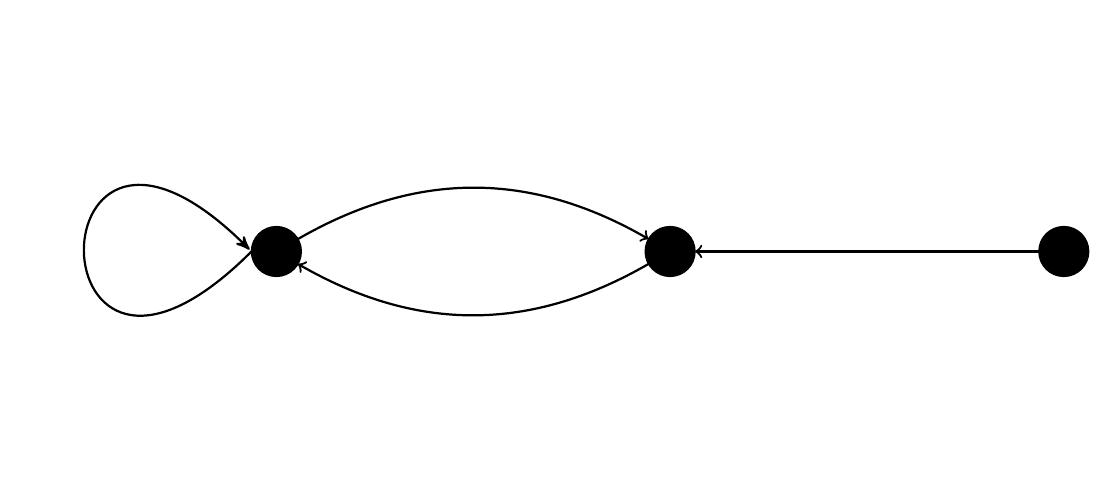
\begin{tikzpicture}   
\tikzset{ 
  VertexStyle/.append style = { fill=black,shape=circle },
  EdgeStyle/.append style = {->, bend left} }
\SetGraphUnit{5}
\Vertex{A}   
\EA(A){B}   
\EA(B){C}   
\Edge[](A)(B)   
\Edge[](B)(A)   
\Loop[dist = 4cm, dir = NO](A.west)
\tikzset{EdgeStyle/.append style = {bend left = 0}}
\Edge[](C)(B)   
\end{tikzpicture}

\caption{Example of a directed graph\label{fig:directed_graph_example}}
\end{figure}


In this chapter, we will build two directed and two undirected graphs:
\begin{itemize}
\item An empty (directed) graph, which is the default type: see chapter
\ref{sub:create_empty_directed_graph}
\item An empty (undirected) graph: see chapter \ref{sub:create_empty_undirected_graph}
\item A two-state Markov chain, a directed graph with two vertices and four
edges, chapter \ref{sub:create_markov_chain_graph}
\item $K_{2}$, an undirected graph with two vertices and one edge, chapter
\ref{sub:create_k2_graph}
\end{itemize}
Creating an empty graph may sound trivial, it is not, thanks to the
versatility of the Boost.Graph library.

In the process of creating graphs, some basic (sometimes bordering
trivial) functions are encountered:
\begin{itemize}
\item Counting the number of vertices: see chapter \ref{sub:get_n_vertices}
\item Counting the number of edges: see chapter \ref{sub:get_n_edges}
\item Adding a vertex: see chapter \ref{sub:add_vertex}
\item Getting all vertices: see chapter \ref{sub:get_vertices}
\item Getting all vertex descriptors: see chapter \ref{sub:get_vertex_descriptors}
\item Adding an edge: see chapter \ref{sub:add_edge}
\item Getting all edges: see chapter \ref{sub:get_edges}
\item Getting all edge descriptors: see chapter \ref{sub:get_edge_descriptors}
\end{itemize}
These functions are mostly there for completion and showing which
data types are used.

The chapter also introduces some important concepts:
\begin{itemize}
\item Vertex descriptors: see chapter \ref{sub:Vertex-descriptors}
\item Edge insertion result: see chapter \ref{sub:boost::add_edge result}
\item Edge descriptors: see chapter \ref{sub:Edge-descriptors}
\end{itemize}

\subsection{Creating an empty (directed) graph\label{sub:create_empty_directed_graph}\index{Create an empty directed graph}\index{Empty directed graph, create}}

Let's create an empty graph!

Algorithm \ref{alg:create_empty_directed_graph} shows the function
to create an empty graph. 

\begin{algorithm}[H]
\lstinputlisting[breaklines=true,language={C++}]{create_empty_directed_graph.impl}

\caption{Creating an empty (directed) graph\index{create_empty_directed_graph@create\_empty\_directed\_graph}\label{alg:create_empty_directed_graph}}
\end{algorithm}


The code consists out of an \#include and a function definition. The
\#include\index{#include@\#include} tells the compiler to read the
header file 'adjacency\_list.hpp'. A header file\index{header file}
(often with a '.h' or '.hpp' extension) contains class and functions
declarations and/or definitions. The header file 'adjacency\_list.hpp'
contains the boost::adjacency\_list class definition. Without including
this file, you will get compile errors like 'definition of boost::adjacency\_list
unknown'%
\footnote{In practice, these compiler error messages will be longer, bordering
the unreadable%
}. The function 'create\_empty\_directed\_graph' has:
\begin{itemize}
\item a return type: The return type is 'boost::adjacency\_list<>', that
is a 'boost::adjacency\_list with all template arguments set at their
defaults
\item a noexcept specification\index{noexcept specification}: the function
should not throw%
\footnote{if the function would throw because it cannot allocate this little
piece of memory, you are already in big trouble%
}, so it is preferred to mark it noexcept\index{noexcept} (\cite{stroustrup2013}
chapter 13.7).
\item a function body: all the function body does is create a 'boost::adjacency\_list<>'
by calling its constructor, by using the round brackets
\end{itemize}
Algorithm \ref{alg:create_empty_directed_graph_demo} demonstrates
the 'create\_empty\_directed\_graph' function. Note that it includes
a header file with the same name as the function%
\footnote{I do not think it is important to have creative names%
} first, to be able to use it. 'auto' is used, as this is preferred
over explicit type declarations (\cite{stroustrup2013} chapter 31.6).
The keyword 'auto'\index{auto} lets the compiler figure aut\index{Pun intended}
the type itself.

\begin{algorithm}[H]
\lstinputlisting[breaklines=true,language={C++}]{create_empty_directed_graph_demo.impl}

\caption{Demonstration of 'create\_empty\_directed\_graph'\label{alg:create_empty_directed_graph_demo}}
\end{algorithm}


Congratulations, you've just created a boost::adjacency\_list\index{boost::adjacency_list@boost::adjacency\_list}
with its default template arguments. We do not do anything with it
yet, but still, you've just created a graph, in which:
\begin{itemize}
\item The out edges are stored in a std::vector
\item The vertices are stored in a std::vector
\item The edges have a direction
\item The vertices, edges and graph have no properties
\item The edges are stored in a std::list
\end{itemize}
The boost::adjacency\_list is the most commonly used graph type, the
other is the boost::adjacency\_matrix\index{boost::adjacency_matrix@boost::adjacency\_matrix}.
It stores its edges, out edges and vertices in a two different STL\index{STL}%
\footnote{Standard Template Library, the standard library%
} containers. std::vector\index{std::vector} is the container you
should use by default (\cite{stroustrup2013} chapter 31.6, \cite{sutter_and_alexandrescu2004}
chapter 76), as it has constant time look-up and back insertion. The
std::list\index{std::list} is used for storing the edges, as it is
better suited at inserting elements at any position.

I use const\index{const} to store the empty graph as we do not modify
it. Correct use of const is called const-correct. Prefer to be const-correct\index{const-correctness}
(\cite{stroustrup1997} chapter 7.9.3, \cite{stroustrup2013} chapter
12.7, \cite{meyers2005effective} item 3, \cite{hollingworth2000cpp_builder_dev_guide}
chapter 3, \cite{sutter_and_alexandrescu2004} item 15, \cite{cline1998cpp_faqs}
FAQ 14.05, \cite{eckel2002thinking_cpp} item 8, \cite{lakos1996large}
9.1.6). 


\subsection{Creating an empty undirected graph\label{sub:create_empty_undirected_graph}\index{Create an empty graph}\index{Empty graph, create}}

Let's create another empty graph! This time, we even make it undirected!

Algorith \ref{alg:create_empty_undirected_graph} shows how to create
an undirected graph.

\begin{algorithm}[H]
\lstinputlisting[breaklines=true,language={C++}]{create_empty_undirected_graph.impl}

\caption{Creating an empty undirected graph\index{create_empty_undirected_graph@create\_empty\_undirected\_graph}\label{alg:create_empty_undirected_graph}}
\end{algorithm}


Algorithm \ref{alg:create_empty_undirected_graph_demo} demonstrates
the 'create\_empty\_undirected\_graph' function.

\begin{algorithm}[H]
\lstinputlisting[breaklines=true,language={C++}]{create_empty_undirected_graph_demo.impl}

\caption{Demonstration of 'create\_empty\_undirected\_graph'\label{alg:create_empty_undirected_graph_demo}}
\end{algorithm}


Congratulations, with algorithm \ref{alg:create_empty_undirected_graph_demo},
you've just created an undirected graph in which:
\begin{itemize}
\item The out edges are stored in a std::vector. This way to store out edges
is selected by the first 'boost::vecS'\index{boost::vecS}
\item The vertices are stored in a std::vector. This way to store vertices
is selected by the second 'boost::vecS'\index{boost::vecS}
\item The graph is undirected. This directionality is selected for by the
third template argument, 'boost::undirectedS'\index{boost::undirectedS}
\item Vertices, edges and graph have no properties
\item Edges are stored in a std::list 
\end{itemize}

\subsection{Counting the number of vertices\label{sub:get_n_vertices}\index{Vertices, counting}\index{Counting the number of vertices}}

Let's count all zero vertices of an empty graph!

\begin{algorithm}[H]
\lstinputlisting[breaklines=true,language={C++}]{get_n_vertices.impl}

\caption{Count the number of vertices\index{get_n_vertices@get\_n\_vertices}\label{alg:get_n_vertices}}
\end{algorithm}


The function 'get\_n\_vertices' takes the result of boost::num\_vertices\index{boost::num_vertices@boost::num\_vertices},
converts it to int and checks if there was no range overflow. We do
so, as one should prefer using int (over unsigned int) in an interface
(\cite{lakos1996large} chapter 9.2.2). To do so, in the function
body its first stament, the unsigned int\index{unsigned int}%
\footnote{or '{[}some type{]}' to be precise%
} produced by boost::num\_vertices\index{boost::num_vertices@boost::num\_vertices}
get converted to an int using a static\_cast\index{static_cast@static\_cast}.
This static\_cast cannot always be correct, as an unsigned int can
have twice as high (but only positive) values. Luckily, this can be
detected: if an unsigned int produces a negative int, it was too big
to be stored as such. Using an unsigned int over a (signed) int for
the sake of gaining that one more bit (\cite{stroustrup1997} chapter
4.4) should be avoided. The integer 'n' is initialized using list-initialization,
which is preferred over the other initialization syntaxes (\cite{stroustrup2013}
chapter 17.7.6). 

The assert statement checks if the conversion from unsigned int to
int was successfull. If it was not, the program crashes. Use assert\index{assert}
extensively (\cite{stroustrup1997} chapter 24.5.18, \cite{stroustrup2013}
chapter 30.5, \cite{sutter_and_alexandrescu2004} chapter 68, \cite{mcconnell2004code}
chapter 8.2, \cite{liberty2001sams} hour 24, \cite{lakos1996large}
chapter 2.6).

The function 'get\_n\_vertices' is demonstrated in algorithm \ref{alg:get_n_vertices_demo},
to measure the number of vertices of both the directed and undirected
graph we are already able to create.

\begin{algorithm}[H]
\lstinputlisting[breaklines=true,language={C++}]{get_n_vertices_demo.impl}

\caption{Demonstration of the 'get\_n\_vertices' function\label{alg:get_n_vertices_demo}}
\end{algorithm}


Note that the type of graph does not matter here. One can count the
number of vertices of every graph, as all graphs have vertices. Boost.Graph
is very good at detecting operations that are not allowed, during
compile time.


\subsection{Counting the number of edges\label{sub:get_n_edges}\index{Edges, counting}\index{Counting the number of edges}}

Let's count all zero edges of an empty graph!

This is very similar to the previous chapter, only it uses boost::num\_edges\index{boost::num_edges@boost::num\_edges}
instead:

\begin{algorithm}[H]
\lstinputlisting[breaklines=true,language={C++}]{get_n_edges.impl}

\caption{Count the number of edges\index{get_n_edges@get\_n\_edges}\label{alg:get_n_edges}}
\end{algorithm}


For the rationale behind this, see the previous chapter.

The function 'get\_n\_edges' is demonstrated in algorithm \ref{alg:get_n_edges_demo},
to measure the number of edges of an empty directed and undirected
graph.

\begin{algorithm}[H]
\lstinputlisting[breaklines=true,language={C++}]{get_n_edges_demo.impl}

\caption{Demonstration of the 'get\_n\_edges' function\label{alg:get_n_edges_demo}}
\end{algorithm}



\subsection{Add a vertex\label{sub:add_vertex}\index{Add a vertex}\index{Vertex, add}}

Empty graphs are nice, now its time to add a vertex!

To add a vertex to a graph, the boost::add\_vertex\index{boost::add_vertex@boost::add\_vertex}
function is used as shows in algorithm \ref{alg:add_vertex}:

\begin{algorithm}[H]
\lstinputlisting[breaklines=true,language={C++}]{add_vertex.impl}

\caption{Adding a vertex to a graph\index{add_vertex@add\_vertex}\label{alg:add_vertex}}
\end{algorithm}


Note that boost::add\_vertex (in the 'add\_vertex' function) returns
a vertex descriptor, which is ignored for now. Vertex descriptors
are looked at in more details at the chapter \ref{sub:Vertex-descriptors},
as we need these to add an edge. Algorithm \ref{alg:add_vertex_demo}
shows how to add a vertex to a directed and undirected graph.

\begin{algorithm}[H]
\lstinputlisting[breaklines=true,language={C++}]{add_vertex_demo.impl}

\caption{Demonstration of the 'add\_vertex' function\label{alg:add_vertex_demo}}
\end{algorithm}


This demonstration code creates two empty graphs, adds one vertex
to each and then asserts that the number of vertices in each graph
is one. This works for both types of graphs, as all graphs have vertices.


\subsection{Vertex descriptors\label{sub:Vertex-descriptors}\index{Vertex descriptor}}

A vertex descriptor is a handle to a vertex within a graph. 

Vertex descriptors can be obtained by dereferencing a vertex iterator
(see chapter \ref{sub:get_vertex_descriptors}). To do so, we first
obtain some vertex iterators in chapter \ref{sub:get_vertices}). 

Vertex descriptors are used to:
\begin{itemize}
\item add and edge between two vertices, see chapter \ref{sub:add_edge}
\item obtain properties of vertex a vertex, for example the vertex its out
degrees (chapter \ref{sub:get_vertex_out_degrees}), the vertex its
name (chapter \ref{sub:get_vertex_names}), or a custom vertex property
(chapter \ref{sub:get_vertex_my_vertexes})
\end{itemize}
In this tutorial, vertex descriptors have named prefixed with 'vd\_'\index{vd_@vd\_},
for example 'vd\_1'.


\subsection{Get the vertices\label{sub:get_vertices}}

You cannot get the vertices. This may sound unexpected, as it must
be possible to work on the vertices of a graph. Working on the vertices
of a graph is done throught these steps:
\begin{itemize}
\item Obtain a vertex iterator pair from the graph
\item Dereferencing a vertex iterator to obtain a vertex descriptor
\end{itemize}
boost::vertices\index{boost::vertices} is used to obtain a vertex
iterator pair\index{Vertex iterator pair}, as shown in algorithm
\ref{alg:get_vertices}. The first vertex iterator\index{Vertex iterator}
points to the first vertex (its descriptor, to be precise), the second
points to beyond the last vertex (its descriptor, to be precise).
In this tutorial, vertex iterator pairs have named prefixed with 'vip\_'\index{vip_@vip\_},
for example 'vip\_1'.

\begin{algorithm}[H]
\lstinputlisting[breaklines=true,language={C++}]{get_vertices.impl}

\caption{Get the vertex iterators of a graph\index{get_vertices@get\_vertices}\label{alg:get_vertices}}
\end{algorithm}


This is a somewhat trivial function, as it forwards the function call
to boost::vertices.

These vertex iterators can be dereferenced to obtain the vertex descriptors.
Note that 'get\_vertices' will not be used often in isolation: usually
one obtains the vertex descriptors immediatly. Just for your reference,
algorithm \ref{alg:get_vertices_demo} demonstrates of the 'get\_vertices'
function, by showing that the vertex iterators of an empty graph point
to the same location.

\begin{algorithm}[H]
\lstinputlisting[breaklines=true,language={C++}]{get_vertices_demo.impl}

\caption{Demonstration of 'get\_vertices'\label{alg:get_vertices_demo}}
\end{algorithm}



\subsection{Get all vertex descriptors\label{sub:get_vertex_descriptors}\index{Vertex descriptors, get}}

Vertex descriptors are the way to manipulate those vertices. Let's
go get the all!

Vertex descriptors are obtained from dereferencing vertex iterators.
Algorithm \ref{alg:get_vertex_descriptors} shows how to obtain all
vertex descriptors from a graph.

\begin{algorithm}[H]
\lstinputlisting[breaklines=true,language={C++}]{get_vertex_descriptors.impl}

\caption{Get all vertex descriptors of a graph\index{get_vertex_descriptors@get\_vertex\_descriptors}\label{alg:get_vertex_descriptors}}
\end{algorithm}


This is the first more complex piece of code. In the first lines,
some 'using' statements allow for shorter type names. The function
'vertices'\index{vertices} (not boost::vertices\index{boost::vertices does not exist}!)
returns a vertex iterator pair. The two iterators are extracted, of
which the first iterator, 'i', points to the first vertex, and the
second, 'j', points to beyond the last vertex. In the for-loop, 'i'
loops from begin to end. Dereferencing it produces a vertex descriptor,
which is stored in the std::vector using emplace\_back. Prefer using
emplace\_back (\cite{stroustrup2013} chapter 31.6, items 25 and 27). 

Algorithm \ref{alg:get_vertex_descriptors_demo} demonstrates that
an empty graph has no vertex descriptors:

\begin{algorithm}[H]
\lstinputlisting[breaklines=true,language={C++}]{get_vertex_descriptors_demo.impl}

\caption{Demonstration of 'get\_vertex\_descriptors'\label{alg:get_vertex_descriptors_demo}}
\end{algorithm}


Because all graphs have (vertices and thus) vertex descriptors, the
type of graph is unimportant for this code to compile.


\subsection{Add an edge\label{sub:add_edge}\index{Add an edge}\index{Edge, add}}

To add an edge to a graph, two vertex descriptors are needed. A vertex
descriptor\index{Vertex descriptor} is a handle to the vertex within
a graph (vertex descriptors are looked at in more details in chapter
\ref{sub:Vertex-descriptors}). Algorithm \ref{alg:add_edge} adds
two vertices to a graph, and connects these two using boost::add\_edge\index{boost::add_edge@boost::add\_edge}: 

\begin{algorithm}[H]
\lstinputlisting[breaklines=true,language={C++}]{add_edge.impl}

\caption{Adding (two vertices and) an edge to a graph\index{add_edge@add\_edge}\label{alg:add_edge}}
\end{algorithm}


Algorithm \ref{alg:add_edge} shows how to add an isolated edge to
a graph (instead of allowing for graphs with higher connectivities).
First, two vertices are created, using the function 'boost::add\_vertex'.
'boost::add\_vertex' returns a vertex descriptor (which I prefix with
'vd'\index{vd}), both of which are stored. The vertex descriptors
are used to add an edge to the graph, using 'boost::add\_edge'\index{boost::add_edge@boost::add\_edge}.
'boost::add\_edge'\index{boost::add_edge@boost::add\_edge} returns
returns a std::pair\index{std::pair}, consisting of an edge descriptor
and a boolean success indicator. The success of adding the edge is
checked by an assert statement. Here we assert\index{assert} that
this insertion was successfull. Insertion can fail if an edge is already
present and duplicates are not allowed.

A demonstration of add\_edge is shown in algorith \ref{alg:add_edge_demo},
in which an edge is added to both a directed and undirected graph.

\begin{algorithm}[H]
\lstinputlisting[breaklines=true,language={C++}]{add_edge_demo.impl}

\caption{Demonstration of 'add\_edge'\label{alg:add_edge_demo}}
\end{algorithm}


The graph type is unimportant: as all graph types have vertices and
edges, edges can be added without possible compile problems.


\subsection{boost::add\_edge result\label{sub:boost::add_edge result}\index{boost::add_edge result@boost::add\_edge result}}

When using the function 'boost::add\_edge', a 'std::pair<edge\_descriptor,bool>'
is returned. It contains both the edge descriptor (see chapter \ref{sub:Edge-descriptors})
and a boolean indicating insertion success.

In this tutorial, boost::add\_edge results have named prefixed with
'aer\_'\index{aer_@aer\_}, for example 'aer\_1'.


\subsection{Getting the edges\label{sub:get_edges}}

You cannot get the edges directly. Instead, working on the edges of
a graph is done throught these steps:
\begin{itemize}
\item Obtain an edge iterator pair from the graph
\item Dereference an edge iterator to obtain an edge descriptor
\end{itemize}
'edges\index{edges}' (not boost::edges\index{boost::edges does not exist}!)
is used to obtain an edge iterator pair\index{Edge iterator pair}.
The first edge iterator\index{Edge iterator} points to the first
edge (its descriptor, to be precise), the second points to beyond
the last edge (its descriptor, to be precise). In this tutorial, edge
iterator pairs have named prefixed with 'eip\_'\index{eip_@eip\_},
for example 'eip\_1'. Algoritm \ref{alg:get_edges} shows how to obtain
these:

\begin{algorithm}[H]
\lstinputlisting[breaklines=true,language={C++}]{get_edges.impl}

\caption{Get the edge iterators of a graph\index{get_edges@get\_edges}\label{alg:get_edges}}
\end{algorithm}


This is a somewhat trivial function, as all it does is forward to
function call to 'edges' (not boost::edges\index{boost::edges does not exist}!)
These edge iterators can be dereferenced to obtain the edge descriptors.
Note that this function will not be used often in isolation: usually
one obtains the edge descriptors immediatly.

Algorithm \ref{alg:get_edges_demo} demonstrates 'get\_edges' by showing
that both iterators of the edge iterator pair point to the same location,
when the graph is empty.

\begin{algorithm}[H]
\lstinputlisting[breaklines=true,language={C++}]{get_edges_demo.impl}

\caption{Demonstration of 'get\_edges'\label{alg:get_edges_demo}}
\end{algorithm}



\subsection{Edge descriptors\label{sub:Edge-descriptors}\index{Edge descriptor}}

An edge descriptor is a handle to an edge within a graph. They are
similar to vertex descriptors (chapter \ref{sub:Vertex-descriptors}). 

Edge descriptors are used to obtain the name, or other properties,
of an edge

In this tutorial, edge descriptors have named prefixed with 'ed\_'\index{ed_@ed\_},
for example 'ed\_1'.


\subsection{Get all edge descriptors\label{sub:get_edge_descriptors}\index{Edge descriptors, get}\index{Get edge descriptors}}

Obtaining all edge descriptors is similar to getting all vertex descriptors
(algorithm \ref{alg:get_vertex_descriptors}):

\begin{algorithm}[H]
\lstinputlisting[breaklines=true,language={C++}]{get_edge_descriptors.impl}

\caption{Get all edge descriptors of a graph\index{get_edge_descriptors@get\_edge\_descriptors}\label{alg:get_edge_descriptors}}
\end{algorithm}


The only difference is that instead of the function 'vertices' (not
boost::vertices\index{boost::vertices does not exist}!), 'edges'\index{edges}
(not boost::edges\index{boost::edges does not exist}!) is used. 

Algorithm \ref{alg:get_edge_descriptors_demo} demonstrates the 'get\_edge\_descriptor',
by showing that empty graphs do not have any edge descriptors.

\begin{algorithm}[H]
\lstinputlisting[breaklines=true,language={C++}]{get_edge_descriptors_demo.impl}

\caption{Demonstration of get\_edge\_descriptors\label{alg:get_edge_descriptors_demo}}
\end{algorithm}



\subsection{Creating a directed graph\label{sub:create_markov_chain_graph}\index{Create directed graph}\index{Directed graph, create}}

Finally, we are going to create a directed graph! 

This directed graph is a two-state Markov chain, with two vertices
and four edges, as depicted in figure \ref{fig:create_markov_chain}:

\begin{figure}[H]
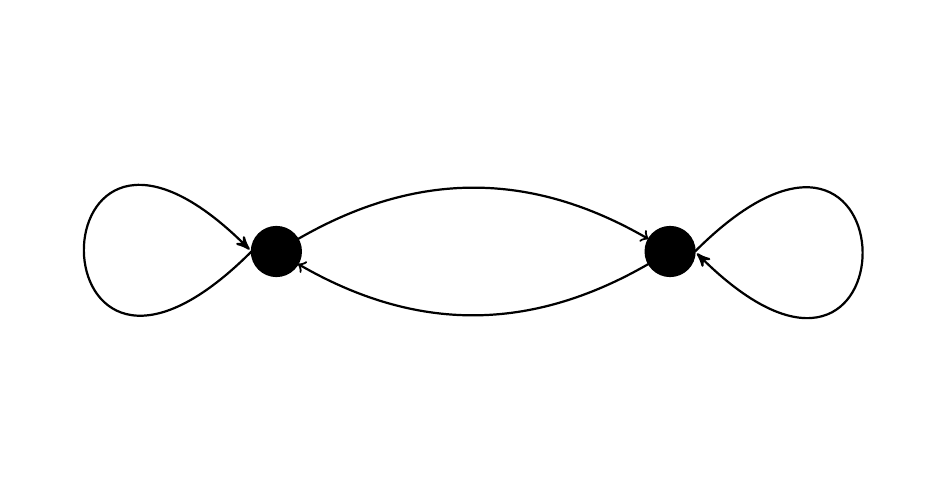
\begin{tikzpicture}   
\tikzset{ 
  VertexStyle/.append style = { fill=black,shape=circle },
  EdgeStyle/.append style = {->, bend left} }
\SetGraphUnit{5}
\Vertex{A}   
\EA(A){B}   
\Edge[](A)(B)   
\Edge[](B)(A)   
\Loop[dist = 4cm, dir = NO](A.west)
\Loop[dist = 4cm, dir = SO](B.east)
\end{tikzpicture}

\caption{The two-state Markov chain\label{fig:create_markov_chain}}
\end{figure}


Note that directed graphs can have edges that start and end in the
same vertex. These are called self-loops.

To create this two-state Markov chain, the following code can be used:

\begin{algorithm}[H]
\lstinputlisting[breaklines=true,language={C++}]{create_markov_chain.impl}

\caption{Creating the two-state Markov chain as depicted in figure \ref{fig:create_markov_chain}\index{create_markov_chain@create\_markov\_chain}\label{alg:create_markov_chain_graph}}
\end{algorithm}


To save defining the type, we call the 'create\_empty\_directed\_graph'
function. The vertex descriptors (see chapter \ref{sub:Vertex-descriptors})
created by two boost::add\_vertex\index{boost::add_vertex@boost::add\_vertex}
calls are stored to add an edge to the graph. Then boost::add\_edge\index{boost::add_edge@boost::add\_edge}
is called four times. Every time, its return type (see chapter \ref{sub:boost::add_edge result})
is checked for a successfull insertion.

Note that the graph lacks all properties: nodes do not have names,
nor do edges.

Algorithm \ref{create_markov_chain_demo} demonstrates the 'create\_markov\_chain\_graph'
function and checks if it has the correct amount of edges and vertices.

\begin{algorithm}[H]
\lstinputlisting[breaklines=true,language={C++}]{create_markov_chain_demo.impl}

\caption{Demonstration of the 'create\_markov\_chain' \label{create_markov_chain_demo}}
\end{algorithm}



\subsubsection{The .dot file of a two-state Markov chain\label{sub:create_markov_chain.dot}}

Running a bit ahead, this graph can be converted to a .dot file (using
algorithm \ref{alg:save_graph_to_dot}) created is displayed in algorithm
\ref{alg:create_markov_chain.dot}:

\begin{algorithm}[H]
\verbatiminput{create_markov_chain.dot}

\caption{.dot file created from the 'create\_markov\_chain\_graph' function
(algorithm \ref{alg:create_markov_chain_graph}), converted from graph
to .dot file using algorithm \ref{alg:save_graph_to_dot}\label{alg:create_markov_chain.dot}}
\end{algorithm}


From the .dot file one can already see that the graph is directed,
because:
\begin{itemize}
\item The first word, 'digraph', denotes a directed graph (where 'graph'
would have indicated an undirectional graph)
\item The edges are written as '->' (where undirected connections would
be written as '--')
\end{itemize}

\subsubsection{The .svg file of a two-state Markov chain\label{sub:create_markov_chain.svg}}

The .svg file of this graph is shown in figure \ref{fig:create_markov_chain.svg}:

\begin{figure}[H]
\includegraphics{create_markov_chain}

\caption{.svg file created from the 'create\_markov\_chain' function (algorithm
\ref{alg:create_markov_chain_graph}) its .dot file and converted
from .dot file to .svg using algorithm \ref{alg:convert_dot_to_svg}\label{fig:create_markov_chain.svg}}
\end{figure}


Also this figure shows that the graph in directed, as the edges have
arrow heads. Note that the .svg is displayed as if the nodes have
names. This is not the case: here, the node indices are shown.


\subsection{Creating $K_{2}$, a fully connected undirected graph with two vertices\label{sub:create_k2_graph}\index{Create $K_{2}$}\index{$K_{2}$, create}}

Finally, we are going to create a graph!

To create a fully connected undirected graph with two vertices (also
called $K_{2}$), one needs two vertices and one (undirected) edge,
as depicted in figure \ref{fig:k2_graph}.

\begin{figure}[H]
\tikz 
\draw[thick] 
  (0,0) node[fill=black,shape=circle,text=white] {} 
    -- (5,1) node[fill=black,shape=circle,text=white] {} 
;

\caption{$K_{2}$: a fully connected undirected graph with two vertices\label{fig:k2_graph}}
\end{figure}


To create $K_{2}$, the following code can be used:

\begin{algorithm}[H]
\lstinputlisting[breaklines=true,language={C++}]{create_k2_graph.impl}

\caption{Creating $K_{2}$ as depicted in figure \ref{fig:k2_graph}\index{create_k2_graph@create\_k2\_graph}\label{alg:create_k2_graph}}
\end{algorithm}


This code is very similar to the 'add\_edge' function (algorithm \ref{alg:add_edge}).
To save defining the type, we call the 'create\_empty\_undirected\_graph'
function. The vertex descriptors (see chapter \ref{sub:Vertex-descriptors})
created by two boost::add\_vertex\index{boost::add_vertex@boost::add\_vertex}
calls are stored to add an edge to the graph. From boost::add\_edge\index{boost::add_edge@boost::add\_edge}
its return type (see chapter \ref{sub:boost::add_edge result}), it
is only checked that insertion has been successfull.

Note that the graph lacks all properties: nodes do not have names,
nor do edges.

Algorithm \ref{alg:create_k2_graph_demo} demonstrates how to 'create\_k2\_graph'
and checks if it has the correct amount of edges and vertices.

\begin{algorithm}[H]
\lstinputlisting[breaklines=true,language={C++}]{create_k2_graph_demo.impl}

\caption{Demonstration of 'create\_k2\_graph' \label{alg:create_k2_graph_demo}}
\end{algorithm}



\subsubsection{The .dot file of $K_{2}$ , a fully connected undirected graph with
two vertices\label{sub:create_k2.dot}}

Running a bit ahead, this graph can be converted to the .dot file
as shown in algorithm \ref{alg:create_k2_graph.dot}:

\begin{algorithm}[H]
\verbatiminput{create_k2_graph.dot}

\caption{.dot file created from the 'create\_k2\_graph' function (algorithm
\ref{alg:create_k2_graph}), converted from graph to .dot file using
algorithm \ref{alg:save_graph_to_dot}\label{alg:create_k2_graph.dot}}
\end{algorithm}


From the .dot file one can already see that the graph is undirected,
because:
\begin{itemize}
\item The first word, 'graph', denotes an undirected graph (where 'digraph'
would have indicated a directional graph)
\item The edge between 0 and 1 is written as '--' (where directed connections
would be written as '->', '<-' or '<>')
\end{itemize}

\subsubsection{The .svg file of $K_{2}$ , a fully connected undirected graph with
two vertices\label{sub:create_k2.svg}}

Continuing to running a bit ahead, this .dot file can be converted
to the .svg as shown in figure \ref{fig:create_k2_graph.svg}:

\begin{figure}[H]
\includegraphics{create_k2_graph}

\caption{.svg file created from the 'create\_k2\_graph' function (algorithm
\ref{alg:create_k2_graph}) its .dot file, converted from .dot file
to .svg using algorithm \ref{alg:convert_dot_to_svg}\label{fig:create_k2_graph.svg}}
\end{figure}


Also this figure shows that the graph in undirected, otherwise the
edge would have one or two arrow heads. Note that the .svg is displayed
as if the nodes have names. This is not the case: here, the node indices
are shown.


\section{Working with graphs without vertices}

Here we'll do some basic stuff:
\begin{itemize}
\item Getting the vertices' out degrees: see chapter \ref{sub:get_vertex_out_degrees}
\item Saving a graph without properties to .dot file: see chapter \ref{sub:save_graph_to_dot}
\item Loading an undirected graph without properties from .dot file: see
chapter \ref{sub:load_undirected_graph_from_dot}
\item Loading a directed graph without properties from .dot file: see chapter
\ref{sub:load_directed_graph_from_dot}
\end{itemize}

\subsection{Getting the vertices' out degree\label{sub:get_vertex_out_degrees}}

As a bonus chapter, let's measure the out degree of all vertices in
a graph. The out degree of a vertex is the number of edges that originate
at it. 

The number of connections is called the 'degree' of the vertex. There
are three types of degrees:
\begin{itemize}
\item in degree: the number of incoming connections, using boost::in\_degree\index{boost::in_degree@boost::in\_degree}
\item out degree: the number of outgoing connections, using boost::in\_degree\index{boost::out_degree@boost::out\_degree}
\item degree: sum of the in degree and out degree, using boost::in\_degree\index{boost::degree}
\end{itemize}
Algorithm \ref{alg:get_vertex_out_degrees} shows how to obtain these:

\begin{algorithm}[H]
\lstinputlisting[breaklines=true,language={C++}]{get_vertex_out_degrees.impl}

\caption{Get the vertices' out degrees\index{get_vertex_out_degrees@get\_vertex\_out\_degrees}\label{alg:get_vertex_out_degrees}}
\end{algorithm}


The structure of this algorithm is similar to get\_vertex\_descriptors
(algorithm \ref{alg:get_vertex_descriptors}), except that the out
degrees from the vertex descriptors are stored. The out degree of
a vertex iterator is obtained from the function 'out\_degree'\index{out_degree@out\_degree}
(not boost::out\_degree\index{boost::out_degree does not exist@boost::out\_degree does not exist}!). 

Albeit that the $K_{2}$ graph and the two-state Markov chain are
rather simple, we can use it to demonstrate 'get\_vertex\_out\_degrees'
on, as shown in algorithm \ref{alg:get_vertex_out_degrees_demo}.

\begin{algorithm}[H]
\lstinputlisting[breaklines=true,language={C++}]{get_vertex_out_degrees_demo.impl}

\caption{Demonstration of the 'get\_vertex\_out\_degrees' function\index{get_vertex_out_degrees_demo@get\_vertex\_out\_degrees\_demo}\label{alg:get_vertex_out_degrees_demo}}
\end{algorithm}


It is expected that $K_{2}$ has one out-degree for every vertex,
where the two-state Markov chain is expected to have two out-degrees
per vertex.


\subsection{Storing a graph as a .dot\label{sub:save_graph_to_dot}\index{Save graph as .dot}\index{Create .dot from graph} }

Graph are easily saved to a file, thanks to Graphviz. Graphviz (short
for Graph Visualization Software) is a package of open-source tools
for drawing graphs. It uses the DOT language for describing graphs,
and these are commonly stored in (plain-text) .dot files:

\begin{algorithm}[H]
\lstinputlisting[breaklines=true,language={C++}]{save_graph_to_dot.impl}

\caption{Storing a graph as a .dot file\index{save_graph_to_dot@save\_graph\_to\_dot}\label{alg:save_graph_to_dot}}
\end{algorithm}


All the code does is create an std::ofstream\index{std::ofstream}
(an output-to-file stream) and use boost::write\_graphviz\index{boost::write_graphviz@boost::write\_graphviz}
to write the DOT description of our graph to that stream. Instead
of 'std::ofstream', one could use std::cout\index{std::cout} (a related
output stream) to display the DOT language on screen directly.

Algorithm \ref{alg:save_graph_to_dot_demo} shows how to use the 'save\_graph\_to\_dot'
function:

\begin{algorithm}[H]
\lstinputlisting[breaklines=true,language={C++}]{save_graph_to_dot_demo.impl}

\caption{Demonstration of the 'save\_graph\_to\_dot' function\index{save_graph_to_dot_demo@save\_graph\_to\_dot\_demo}\label{alg:save_graph_to_dot_demo}}
\end{algorithm}


When using the 'save\_graph\_to\_dot' function (algorithm \ref{alg:save_graph_to_dot}),
only the structure of the graph is saved: all other properties like
names are not stored. Algorithm \ref{alg:save_named_vertices_graph_to_dot}
shows how to do so.


\subsection{Loading an undirected graph from a .dot\label{sub:load_undirected_graph_from_dot}\index{Load undirected graph from .dot}\index{Create undirected graph from .dot} }

Before loading a graph from file, one needs to specify a type of graph.
In this example, an undirected graph is loaded, as shown in algorithm
\ref{alg:load_undirected_graph_from_dot}:

\begin{algorithm}[H]
\lstinputlisting[breaklines=true,language={C++}]{load_undirected_graph_from_dot.impl}

\caption{Loading an undirected graph from a .dot file\index{load_undirected_graph_from_dot@load\_undirected\_graph\_from\_dot}\label{alg:load_undirected_graph_from_dot}}
\end{algorithm}


In this algorithm, first it is checked if the file to load exists,
using the 'is\_regular\_file' function (algorithm \ref{alg:is_regular_file}),
after which a std::ifstream\index{std::ifstream} (input-file-stream)
is opened. Then an empty undirected graph is created. Next to this,
a boost::dynamic\_properties\index{boost::dynamic_properties@boost::dynamic\_properties}
is created with the 'boost::ignore\_other\_properties'\index{boost::ignore_other_properties@boost::ignore\_other\_properties}
in its constructor (using a default constructor here results in the
run-time error 'property not found: node\_id', see chapter \ref{sub:property_not_found_node_id}).
From this and the empty graph, 'boost::read\_graphviz'\index{boost::read_graphviz@boost::read\_graphviz}
is called to build up the graph.

Algorithm \ref{alg:load_undirected_graph_from_dot_demo} shows how
to use the 'load\_undirected\_graph\_from\_dot' function:

\begin{algorithm}[H]
\lstinputlisting[breaklines=true,language={C++}]{load_undirected_graph_from_dot_demo.impl}

\caption{Demonstration of the 'load\_undirected\_graph\_from\_dot' function\index{load_undirected_graph_from_dot_demo@load\_undirected\_graph\_from\_dot\_demo}\label{alg:load_undirected_graph_from_dot_demo}}
\end{algorithm}


This demonstration shows how the $K_{2}$ graph is created using the
'create\_k2\_graph' function (algorithm \ref{alg:create_k2_graph}),
saved and then loaded. The loaded graph is checked to be a $K_{2}$
graph.


\subsection{Loading an directed graph from a .dot\label{sub:load_directed_graph_from_dot}\index{Load directed graph from .dot}\index{Create directed graph from .dot} }

When loading a graph from file, one needs to specify a type of graph.
In this example, an directed graph is loaded, as shown in algorithm
\ref{alg:load_directed_graph_from_dot}:

\begin{algorithm}[H]
\lstinputlisting[breaklines=true,language={C++}]{load_directed_graph_from_dot.impl}

\caption{Loading a directed graph from a .dot file\index{load_directed_graph_from_dot@load\_directed\_graph\_from\_dot}\label{alg:load_directed_graph_from_dot}}
\end{algorithm}


In this algorithm, first it is checked if the file to load exists,
using the 'is\_regular\_file' function (algorithm \ref{alg:is_regular_file}),
after which an std::ifstream\index{std::ifstream} is opened. Then
an empty directed graph is created. Next to this, a boost::dynamic\_properties\index{boost::dynamic_properties@boost::dynamic\_properties}
is created with the 'boost::ignore\_other\_properties'\index{boost::ignore_other_properties@boost::ignore\_other\_properties}
in its constructor (using a default constructor here results in the
run-time error 'property not found: node\_id', see chapter \ref{sub:property_not_found_node_id}).
From this and the empty graph, 'boost::read\_graphviz'\index{boost::read_graphviz@boost::read\_graphviz}
is called to build up the graph.

Algorithm \ref{alg:load_directed_graph_from_dot_demo} shows how to
use the 'load\_directed\_graph\_from\_dot' function:

\begin{algorithm}[H]
\lstinputlisting[breaklines=true,language={C++}]{load_directed_graph_from_dot_demo.impl}

\caption{Demonstration of the 'load\_directed\_graph\_from\_dot' function\index{load_directed_graph_from_dot_demo@load\_directed\_graph\_from\_dot\_demo}\label{alg:load_directed_graph_from_dot_demo}}
\end{algorithm}


This demonstration shows how the Markov chain is created using the
'create\_markov\_chain\_graph' function (algorithm \ref{alg:create_markov_chain_graph}),
saved and then loaded. The loaded graph is then checked to be a two-state
Markov chain.


\section{Building graphs with named vertices}

Up until now, the graphs created have had edges and vertices without
any propery. In this chapter, graphs will be created, in which the
vertices can have a name. This name will be of the std::string data
type, but other types are possible as well. There are many more built-in
properties edges and nodes can have (see chapter \ref{sub:all_properties}
for a list).

In this chapter, we will build the following graphs:
\begin{itemize}
\item An empty directed graph that allows for vertices with names: see chapter
\ref{sub:create_empty_directed_named_vertices_graph}
\item An empty undirected graph that allows for vertices with names: see
chapter \ref{sub:create_empty_undirected_named_vertices_graph}
\item Two-state Markov chain with named vertices: see chapter \ref{sub:create_named_vertices_markov_chain}
\item $K_{2}$ with named vertices: see chapter \ref{sub:create_named_vertices_k2_graph}
\end{itemize}
In the process, some basic (sometimes bordering trivial) functions
are shown:
\begin{itemize}
\item Adding a named vertex: see chapter \ref{sub:add_named_vertex}
\item Getting the vertices' names: see chapter \ref{sub:get_vertex_names}
\end{itemize}
These functions are mostly there for completion and showing which
data types are used.


\subsection{Creating an empty directed graph with named vertices\label{sub:create_empty_directed_named_vertices_graph}\index{Create an empty directed graph with named vertices}\index{Named vertices, create empty directed graph}\index{Empty directed graph with named vertices, create}}

Let's create a trivial empty directed graph, in which the vertices
can have a name:

\begin{algorithm}[H]
\lstinputlisting[breaklines=true,language={C++}]{create_empty_directed_named_vertices_graph.impl}

\caption{Creating an empty directed graph with named vertices\index{create_empty_directed_named_vertices_graph@create\_empty\_directed\_named\_vertices\_graph}\label{alg:create_empty_directed_named_vertices_graph}}
\end{algorithm}


This graph:
\begin{itemize}
\item has its out edges stored in a std::vector (due to the first boost::vecS\index{boost::vecS})
\item has its vertices stored in a std::vector (due to the second boost::vecS\index{boost::vecS})
\item is directed (due to the boost::directedS\index{boost::directedS})
\item The vertices have one property: they have a name, that is of data
type std::string (due to the boost::property< boost::vertex\_name\_t,std::string>\index{boost::property}\index{boost::vertex_name_t@boost::vertex\_name\_t}')
\item Edges and graph have no properties
\item Edges are stored in a std::list
\end{itemize}
The boost::adjacency\_list\index{boost::adjacency_list@boost::adjacency\_list}
has a new, fourth template argument 'boost::property< boost::vertex\_name\_t,std::string>\index{boost::property}\index{boost::vertex_name_t@boost::vertex\_name\_t}'.
This can be read as: ``vertices have the property 'boost::vertex\_name\_t',
that is of data type 'std::string'''. Or simply: ``vertices have
a name that is stored as a std::string''.

Algorithm \ref{alg:create_empty_directed_named_vertices_graph_demo}
shows how to create this graph. Note that all the earlier functions
defined in this tutorial keep working as expected.

\begin{algorithm}[H]
\lstinputlisting[breaklines=true,language={C++}]{create_empty_directed_named_vertices_graph_demo.impl}

\caption{Demonstration of the 'create\_empty\_directed\_named\_vertices\_graph'
function \index{create_empty_named_directed_vertices_graph_demo@create\_empty\_named\_directed\_vertices\_graph\_demo}\label{alg:create_empty_directed_named_vertices_graph_demo}}
\end{algorithm}



\subsection{Creating an empty undirected graph with named vertices\label{sub:create_empty_undirected_named_vertices_graph}\index{Create an empty undirected graph with named vertices}\index{Named vertices, create empty undirected graph}\index{Empty undirected graph with named vertices, create}}

Let's create a trivial empty undirected graph, in which the vertices
can have a name:

\begin{algorithm}[H]
\lstinputlisting[breaklines=true,language={C++}]{create_empty_undirected_named_vertices_graph.impl}

\caption{Creating an empty undirected graph with named vertices\index{create_empty_undirected_named_vertices_graph@create\_empty\_undirected\_named\_vertices\_graph}\label{alg:create_empty_undirected_named_vertices_graph}}
\end{algorithm}


There is not much happening in this code, except for returning a boost::adjacency\_list
of the correct type.

This graph:
\begin{itemize}
\item has its out edges stored in a std::vector (due to the first boost::vecS\index{boost::vecS})
\item has its vertices stored in a std::vector (due to the second boost::vecS\index{boost::vecS})
\item is undirected (due to the boost::undirectedS\index{boost::undirectedS})
\item The vertices have one property: they have a name, that is of data
type std::string (due to the boost::property< boost::vertex\_name\_t,std::string>\index{boost::property}\index{boost::vertex_name_t@boost::vertex\_name\_t}')
\item Edges and graph have no properties
\item Edges are stored in a std::list
\end{itemize}
The boost::adjacency\_list\index{boost::adjacency_list@boost::adjacency\_list}
has a new, fourth template argument 'boost::property< boost::vertex\_name\_t,std::string>\index{boost::property}\index{boost::vertex_name_t@boost::vertex\_name\_t}'.
This can be read as: ``vertices have the property 'boost::vertex\_name\_t',
that is of data type 'std::string'''. Or simply: ``vertices have
a name that is stored as a std::string''.

Algorithm \ref{alg:create_empty_undirected_named_vertices_graph_demo}
shows how to create this graph:

\begin{algorithm}[H]
\lstinputlisting[breaklines=true,language={C++}]{create_empty_undirected_named_vertices_graph_demo.impl}

\caption{Demonstration of the 'create\_empty\_undirected\_named\_vertices\_graph'
function \index{create_empty_named_undirected_vertices_graph_demo@create\_empty\_named\_undirected\_vertices\_graph\_demo}\label{alg:create_empty_undirected_named_vertices_graph_demo}}
\end{algorithm}



\subsection{Add a vertex with a name\label{sub:add_named_vertex}\index{Add named vertex}\index{Named vertex, add}\index{Vertex, add named}}

Adding a vertex without a name was trivially easy (see chapter \ref{sub:add_vertex}).
Adding a vertex with a name takes slightly more work, as shown by
algorithm \ref{alg:add_named_vertex}:

\begin{algorithm}[H]
\lstinputlisting[breaklines=true,language={C++}]{add_named_vertex.impl}

\caption{Adding a vertex with a name\index{add_named_vertex@add\_named\_vertex}\label{alg:add_named_vertex}}
\end{algorithm}


Instead of calling 'boost::add\_vertex' with an additional argument
containing the name of the vertex%
\footnote{I am unsure if this would have been a good interface. I am sure I
expected this interface myself. I do see a problem with multiple properties
and the order of initialization, but initialization could simply follow
the same order as the the property list.%
}, multiple things need to be done. When adding a new vertex to the
graph, the vertex descriptor (as describes in chapter \ref{sub:Vertex-descriptors})
is stored. After obtaining the name map from the graph (using 'get(boost::vertex\_name,g)\index{get}\index{boost::vertex_name@boost::vertex\_name}'),
the name of the vertex is set using that vertex descriptor. Note that
'get' has no 'boost::' prepending it, as it lives in the same (global)
namespace the function is in. Using 'boost::get' will not compile\index{boost::get does not exist}.

Using add\_named\_vertex is straightforward, as demonstrated by algorithm
\ref{alg:add_named_vertex_demo}.

\begin{algorithm}[H]
\lstinputlisting[breaklines=true,language={C++}]{add_named_vertex_demo.impl}

\caption{Demonstration of 'add\_named\_vertex'\index{add_named_vertex_demo@add\_named\_vertex\_demo}\index{Reference to Superman}\label{alg:add_named_vertex_demo}}
\end{algorithm}



\subsection{Getting the vertices' names\label{sub:get_vertex_names}}

When the vertices of a graph have named vertices, one can extract
them as such:

\begin{algorithm}[H]
\lstinputlisting[breaklines=true,language={C++}]{get_vertex_names.impl}

\caption{Get the vertices' names\index{get_vertex_names@get\_vertex\_names}\label{alg:get_vertex_names}}
\end{algorithm}


This code is very similar to 'get\_vertex\_out\_degrees' (algorithm
\ref{alg:get_vertex_out_degrees}), as also there we iterated through
all vertices, accessing all vertex descriptors sequentially.

The names of the vertices are obtained from a boost::property\_map
and then put into a std::vector. Note that the std::vector has element
type 'std::string', instead of extracting the type from the graph.
If you know how to do so, please email me.

When trying to get the vertices' names from a graph without vertices
with names, you will get the error 'formed reference to void' (see
chapter \ref{sub:formed_reference_to_void}).

Algorithm \ref{alg:get_vertex_names_demo} shows how to add two named
vertices, and check if the added names are retrieved as expected.

\begin{algorithm}[H]
\lstinputlisting[breaklines=true,language={C++}]{get_vertex_names_demo.impl}

\caption{Demonstration of 'get\_vertex\_names'\index{get_vertex_names_demo@get\_vertex\_names\_demo}\label{alg:get_vertex_names_demo}}
\end{algorithm}



\subsection{Creating a Markov chain with named vertices\label{sub:create_named_vertices_markov_chain}\index{Create Markov chain with named vertices}\index{Markov chain with named vertices, create}}

We extend the Markov chain of chapter \ref{sub:create_markov_chain_graph}
by naming the vertices $Sunny$ and $Rainy$, as depicted in figure
\ref{fig:named_vertices_markov_chain}:

\begin{figure}[H]
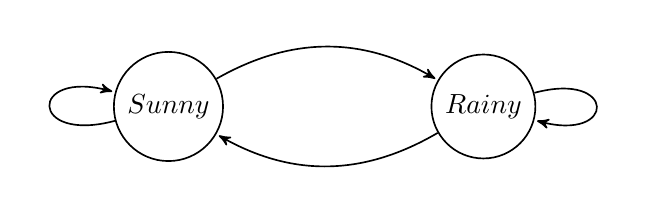
\begin{tikzpicture}[->,>=stealth',shorten >=1pt,auto,node distance=4cm, semithick]   
\tikzstyle{every state}=[]
\node[state] (A)              {$Sunny$};   
\node[state] (B) [right of=A] {$Rainy$};   
\path (A) edge [bend  left] node {} (B)
      (A) edge [loop  left] node {} (A)
      (B) edge [bend  left] node {} (A)
      (B) edge [loop right] node {} (B); 
\end{tikzpicture}

\caption{A two-state Markov chain where the vertices have texts $Sunny$ and
$Rainy$\label{fig:named_vertices_markov_chain}}
\end{figure}


To create this Markov chain, the following code can be used:

\begin{algorithm}[H]
\lstinputlisting[breaklines=true,language={C++}]{create_named_vertices_markov_chain.impl}

\caption{Creating a Markov chain with named vertices as depicted in figure
\ref{fig:named_vertices_markov_chain}\index{create_named_vertices_markov_chain@create\_named\_vertices\_markov\_chain}\label{alg:create_named_vertices_markov_chain}}
\end{algorithm}


Most of the code is a repeat of algorithm \ref{alg:create_markov_chain_graph},
'create\_markov\_chain\_graph'. In the end, the names are obtained
as a boost::property\_map and set to the desired values.

Also the demonstration code (algorithm \ref{alg:create_named_vertices_markov_chain_demo})
is very similar to the demonstration code of the 'create\_markov\_chain\_graph'
function (algorithm \ref{create_markov_chain_demo}).

\begin{algorithm}[H]
\lstinputlisting[breaklines=true,language={C++}]{create_named_vertices_markov_chain_demo.impl}

\caption{Demonstrating the 'create\_named\_vertices\_markov\_chain' function\label{alg:create_named_vertices_markov_chain_demo}}
\end{algorithm}



\subsubsection{The .dot file\label{sub:create_named_vertices_markov_chain.dot}}

\begin{algorithm}[H]
\verbatiminput{create_named_vertices_markov_chain.dot}

\caption{.dot file created from the 'create\_named\_vertices\_markov\_chain'
function (algorithm \ref{alg:create_named_vertices_markov_chain}),
converted from graph to .dot file using algorithm \ref{alg:save_graph_to_dot}\label{alg:create_named_vertices_markov_chain.dot}}
\end{algorithm}



\subsubsection{The .svg file\label{sub:create_named_vertices_markov_chain.svg}}

\begin{figure}[H]
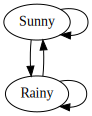
\includegraphics{create_named_vertices_markov_chain}

\caption{.svg file created from the 'create\_named\_vertices\_markov\_chain'
function (algorithm \ref{alg:create_named_vertices_markov_chain})
its .dot file, converted from .dot file to .svg using algorithm \ref{alg:convert_dot_to_svg}\label{fig:create_named_vertices_markov_chain.svg}}
\end{figure}



\subsection{Creating $K_{2}$ with named vertices\label{sub:create_named_vertices_k2_graph}\index{Create $K_{2}$ with named vertices}\index{$K_{2}$ with named vertices, create}}

We extend $K_{2}$ of chapter \ref{sub:create_k2_graph} by naming
the vertices $A$ and $B$, as depicted in figure \ref{fig:named_vertices_k2_graph}:

\begin{figure}[H]
\tikz 
\draw[thick] 
  (0,0) node[fill=black,shape=circle,text=white] {$A$} 
    -- (5,0) node[fill=black,shape=circle,text=white] {$B$} 
;

\caption{$K_{2}$: a fully connected graph with two vertices with the text
$A$ and $B$\label{fig:named_vertices_k2_graph}}
\end{figure}


To create $K_{2}$, the following code can be used:

\begin{algorithm}[H]
\lstinputlisting[breaklines=true,language={C++}]{create_named_vertices_k2_graph.impl}

\caption{Creating $K_{2}$ with named vertices as depicted in figure \ref{fig:named_vertices_k2_graph}\index{create_named_vertices_k2_graph@create\_named\_vertices\_k2\_graph}\label{alg:create_named_vertices_k2_graph}}
\end{algorithm}


Most of the code is a repeat of algorithm \ref{alg:create_k2_graph}.
In the end, the names are obtained as a boost::property\_map and set
to the desired names.

Also the demonstration code (algorithm \ref{alg:create_named_vertices_k2_graph_demo})
is very similar to the demonstration code of the create\_k2\_graph
function (algorithm \ref{alg:create_k2_graph}).

\begin{algorithm}[H]
\lstinputlisting[breaklines=true,language={C++}]{create_named_vertices_k2_graph_demo.impl}

\caption{Demonstrating the 'create\_k2\_graph' function\label{alg:create_named_vertices_k2_graph_demo}}
\end{algorithm}



\subsubsection{The .dot file\label{sub:create_named_vertices_k2.dot}}

\begin{algorithm}[H]
\verbatiminput{create_named_vertices_k2.dot}

\caption{.dot file created from the 'create\_named\_vertices\_k2' function
(algorithm \ref{alg:create_named_vertices_k2_graph}), converted from
graph to .dot file using algorithm \ref{alg:save_graph_to_dot}\label{alg:create_named_vertices_k2_graph.dot}}
\end{algorithm}



\subsubsection{The .svg file\label{sub:create_named_vertices_k2_graph.svg}}

\begin{figure}[H]
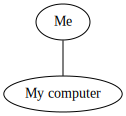
\includegraphics{create_named_vertices_k2_graph}

\caption{.svg file created from the 'create\_named\_vertices\_k2\_graph' function
(algorithm \ref{alg:create_named_vertices_markov_chain}) its .dot
file, converted from .dot file to .svg using algorithm \ref{alg:convert_dot_to_svg}\label{fig:create_named_vertices_k2_graph.svg}}
\end{figure}



\section{Working with graphs with named vertices}

When vertices have names, this name gives a way to find a vertex and
working with it. This chapter shows some basic operations on graphs
with named vertices.
\begin{itemize}
\item Check if there exists a vertex with a certain name: chapter \ref{sub:has_vertex_with_name}
\item Find a vertex by its name: chapter \ref{sub:find_first_vertex_with_name}
\item Get a named vertex its degree, in degree and out degree: chapter:
\ref{sub:get_first_vertex_with_name_out_degree}
\item Get a vertex its name from its vertex descriptor: chapter \ref{sub:get_vertex_name}
\item Set a vertex its name using its vertex descriptor: chapter \ref{sub:set_vertex_name}
\item Setting all vertices' names: chapter \ref{sub:set_vertex_names}
\item Clear a named vertex its edges: chapter \ref{sub:clear_first_vertex_with_name}
\item Remove a named vertex: chapter \ref{sub:remove_first_vertex_with_name}
\item Removing an edge between two named vertices: chapter \ref{sub:remove_edge_between_vertices_with_names}
\item Storing an directed/undirected graph with named vertices as a .dot
file: chapter \ref{sub:save_named_vertices_graph_to_dot}
\item Loading a directed graph with named vertices from a .dot file: chapter
\ref{sub:load_directed_named_vertices_graph_from_dot}
\end{itemize}
Especially chapter \ref{sub:find_first_vertex_with_name} is important:
'find\_first\_vertex\_by\_name' shows how to obtain a vertex descriptor,
which is used in later algorithms.


\subsection{Check if there exists a vertex with a certain name\label{sub:has_vertex_with_name}}

Before modifying our vertices, let's first determine if we can find
a vertex by its name in a graph. After obtaing a name map, we obtain
the vertex iterators, dereference these to obtain the vertex descriptors
and then compare each vertex its name with the one desired.

\begin{algorithm}[H]
\lstinputlisting[breaklines=true,language={C++}]{has_vertex_with_name.impl}

\caption{Find if there is vertex with a certain name\index{has_vertex_with_name@has\_vertex\_with\_name}\label{alg:has_vertex_with_name}}
\end{algorithm}


This function can be demonstrated as in algorithm \ref{alg:has_vertex_with_name_demo},
where a certain name cannot be found in an empty graph. After adding
the desired name, it is found.

\begin{algorithm}[H]
\lstinputlisting[breaklines=true,language={C++}]{has_vertex_with_name_demo.impl}

\caption{Demonstration of the 'has\_vertex\_with\_name' function\index{has_vertex_with_name_demo@has\_vertex\_with\_name\_demo}\label{alg:has_vertex_with_name_demo}}
\end{algorithm}


Note that this function only finds if there is at least one vertex
with that name: it does not tell how many vertices with that name
exist in the graph.


\subsection{Find a vertex by its name\label{sub:find_first_vertex_with_name}}

Where STL functions work with iterators, here we obtain a vertex descriptor
(see chapter \ref{sub:Vertex-descriptors}) to obtain a handle to
the desired vertex. Algorithm \ref{alg:find_first_vertex_with_name}
shows how to obtain a vertex descriptor to the first (name) vertex
found with a specific name.

\begin{algorithm}[H]
\lstinputlisting[breaklines=true,language={C++}]{find_first_vertex_with_name.impl}

\caption{Find the first vertex by its name\index{find_first_vertex_by_name@find\_first\_vertex\_by\_name}\label{alg:find_first_vertex_with_name}}
\end{algorithm}


With the vertex descriptor obtained, one can read and modify the vertex
and the edges surrounding it. Algorithm \ref{alg:find_first_vertex_with_name_demo}
shows some examples of how to do so.

\begin{algorithm}[H]
\lstinputlisting[breaklines=true,language={C++}]{find_first_vertex_with_name_demo.impl}

\caption{Demonstration of the 'find\_first\_vertex\_by\_name' function\index{find_first_vertex_by_name_demo@find\_first\_vertex\_by\_name\_demo}\label{alg:find_first_vertex_with_name_demo}}
\end{algorithm}



\subsection{Get a (named) vertex its degree, in degree and out degree\label{sub:get_first_vertex_with_name_out_degree}}

We already obtained all out degrees of all vertices in chapter \ref{sub:get_vertex_out_degrees}
by just collecting all vertex descriptors. Here, we will search for
a vertex with a certain name, obtain its vertex descriptor and find
the number of connections it has. 

With a vertex descriptor, we can read a vertex its types of degrees.
Algorithm \ref{alg:find_first_vertex_with_name} shows how to find
a vertex, obtain its vertex descriptor and then obtain the out degree
from it.

\begin{algorithm}[H]
\lstinputlisting[breaklines=true,language={C++}]{get_first_vertex_with_name_out_degree.impl}

\caption{Get the first vertex with a certain name its out degree from its vertex
descriptor\index{get_first_vertex_with_name_out_degree@get\_first\_vertex\_with\_name\_out\_degree}\label{alg:get_first_vertex_with_name_out_degree}}
\end{algorithm}


Algorithm \ref{alg:get_first_vertex_with_name_out_degree_demo} shows
how to use this function.

\begin{algorithm}[H]
\lstinputlisting[breaklines=true,language={C++}]{get_first_vertex_with_name_out_degree_demo.impl}

\caption{Demonstration of the 'get\_first\_vertex\_with\_name\_out\_degree'
function\index{get_first_vertex_with_name_out_degree_demo@get\_first\_vertex\_with\_name\_out\_degree\_demo}\label{alg:get_first_vertex_with_name_out_degree_demo}}
\end{algorithm}



\subsection{Get a vertex its name from its vertex descriptor\label{sub:get_vertex_name}}

This may seem a trivial paragraph, as chapter \ref{sub:get_vertex_names}
describes the 'get\_vertex\_names' algorithm, in which we get all
vertices' names. But it does not allow to first find a vertex of interest
and subsequently getting only that one its name.

To obtain the name from a vertex descriptor, one needs to pull out
the name map and then look up the vertex of interest (I like to compare
it as such: the vertex descriptor is a last name, the name map is
a phone book, the desired info a phone number).

\begin{algorithm}[H]
\lstinputlisting[breaklines=true,language={C++}]{get_vertex_name.impl}

\caption{Get a vertex its name from its vertex descriptor\index{get_vertex_name@get\_vertex\_name}\label{alg:get_vertex_name}}
\end{algorithm}


To use 'get\_vertex\_name', one first needs to obtain a vertex descriptor.
Algorithm \ref{alg:get_vertex_name_demo} shows a simple example:

\begin{algorithm}[H]
\lstinputlisting[breaklines=true,language={C++}]{get_vertex_name_demo.impl}

\caption{Demonstration if the 'get\_vertex\_name' function\index{get_vertex_name_demo@get\_vertex\_name\_demo}\label{alg:get_vertex_name_demo}}
\end{algorithm}



\subsection{Set a (named) vertex its name from its vertex descriptor\label{sub:set_vertex_name}}

If you know how to get the name from a vertex descriptor, setting
it is just as easy, as shown in algorithm \ref{alg:set_vertex_name}.

\begin{algorithm}[H]
\lstinputlisting[breaklines=true,language={C++}]{set_vertex_name.impl}

\caption{Set a vertex its name from its vertex descriptor\index{set_vertex_name@set\_vertex\_name}\label{alg:set_vertex_name}}
\end{algorithm}


To use 'set\_vertex\_name', one first needs to obtain a vertex descriptor.
Algorithm \ref{alg:set_vertex_name_demo} shows a simple example.

\begin{algorithm}[H]
\lstinputlisting[breaklines=true,language={C++}]{set_vertex_name_demo.impl}

\caption{Demonstration if the 'set\_vertex\_name' function\index{set_vertex_name_demo@set\_vertex\_name\_demo}\label{alg:set_vertex_name_demo}}
\end{algorithm}



\subsection{Setting all vertices' names\label{sub:set_vertex_names}\index{Set vertices names}\index{Vertices, set names}}

When the vertices of a graph have named vertices and you want to set
all their names at once:

\begin{algorithm}[H]
\lstinputlisting[breaklines=true,language={C++}]{set_vertex_names.impl}

\caption{Setting the vertices' names\index{set_vertex_names@set\_vertex\_names}\label{alg:set_vertex_names}}
\end{algorithm}


This is not a very usefull function if the graph is complex. But for
just creating graphs for debugging, it may come in handy.


\subsection{Clear the edges of a named vertex\label{sub:clear_first_vertex_with_name}}

A vertex descriptor can be used to clear all in/out/both edges connected
to a vertex. It is necessary to remove these connections before the
vertex itself can be removed. There are three functions to remove
the edges connected to a vertex:
\begin{itemize}
\item boost::clear\_vertex\index{boost::clear_vertex@boost::clear\_vertex}:
removes all edges to and from the vertex 
\item boost::clear\_out\_edges\index{boost::clear_out_edges@boost::clear\_out\_edges}:
removes all outgoing edges from the vertex (in directed graphs only,
else you will get a 'error: no matching function for call to clear\_out\_edges',
as described in chapter \ref{sub:no_matching_function_for_call_to_clear_out_edges})
\item boost::clear\_in\_edges\index{boost::clear_in_edges@boost::clear\_in\_edges}:
removes all incoming edges from the vertex (in directed graphs only,
else you will get a 'error: no matching function for call to clear\_in\_edges',
as described in chapter \ref{sub:no_matching_function_for_call_to_clear_in_edges})
\end{itemize}
In the algorithm 'clear\_first\_vertex\_with\_name' the 'boost::clear\_vertex'
algorithm is used, as the graph used is undirectional:

\begin{algorithm}[H]
\lstinputlisting[breaklines=true,language={C++}]{clear_first_vertex_with_name.impl}

\caption{Clear the first vertex with a certain name\index{clear_first_vertex_with_name@clear\_first\_vertex\_with\_name}\label{alg:clear_first_vertex_with_name}}
\end{algorithm}


Algorithm \ref{alg:clear_first_vertex_with_name_demo} shows the clearing
of the first named vertex found.

\begin{algorithm}[H]
\lstinputlisting[breaklines=true,language={C++}]{clear_first_vertex_with_name_demo.impl}

\caption{Demonstration of the 'clear\_first\_vertex\_with\_name' function\index{clear_first_vertex_with_name_demo@clear\_first\_vertex\_with\_name\_demo}\label{alg:clear_first_vertex_with_name_demo}}
\end{algorithm}



\subsection{Remove a named vertex\label{sub:remove_first_vertex_with_name}}

A vertex descriptor can be used to remove a vertex from a graph. It
is necessary to remove these connections (e.g. using clear\_first\_vertex\_with\_name',
algorithm \ref{alg:clear_first_vertex_with_name}) before the vertex
itself can be removed. 

Removing a named vertex goes as follows: use the name of the vertex
to get a first vertex descriptor, then call 'boost::remove\_vertex'\index{boost::remove_vertex@boost::remove\_vertex},
shown in algorithm \ref{alg:clear_first_vertex_with_name}.

\begin{algorithm}[H]
\lstinputlisting[breaklines=true,language={C++}]{remove_first_vertex_with_name.impl}

\caption{Remove the first vertex with a certain name\index{remove_first_vertex_with_name@remove\_first\_vertex\_with\_name}\label{alg:remove_first_vertex_with_name}}
\end{algorithm}


Algorithm \ref{alg:remove_first_vertex_with_name_demo} shows the
removal of the first named vertex found.

\begin{algorithm}[H]
\lstinputlisting[breaklines=true,language={C++}]{remove_first_vertex_with_name_demo.impl}

\caption{Demonstration of the 'remove\_first\_vertex\_with\_name' function\index{remove_first_vertex_with_name_demo@remove\_first\_vertex\_with\_name\_demo}\label{alg:remove_first_vertex_with_name_demo}}
\end{algorithm}


Again, be sure that the vertex removed does not have any connections!


\subsection{Removing the edge between two named vertices\label{sub:remove_edge_between_vertices_with_names}}

Instead of looking for an edge descriptor, one can also remove an
edge from two vertex descriptors (which is: the edge between the two
vertices). Removing an edge between two named vertices named edge
goes as follows: use the names of the vertices to get both vertex
descriptors, then call 'boost::remove\_edge'\index{boost::remove_edge@boost::remove\_edge}
on those two, as shown in algorithm \ref{alg:remove_edge_between_vertices_with_names}.

\begin{algorithm}[H]
\lstinputlisting[breaklines=true,language={C++}]{remove_edge_between_vertices_with_names.impl}

\caption{Remove the first edge with a certain name\index{remove_edge_between_vertices_with_names@remove\_edge\_between\_vertices\_with\_names}\label{alg:remove_edge_between_vertices_with_names}}
\end{algorithm}


Algorithm \ref{alg:remove_edge_between_vertices_with_names_demo}
shows the removal of the first named edge found.

\begin{algorithm}[H]
\lstinputlisting[breaklines=true,language={C++}]{remove_edge_between_vertices_with_names_demo.impl}

\caption{Demonstration of the 'remove\_edge\_between\_vertices\_with\_names'
function\label{alg:remove_edge_between_vertices_with_names_demo}}
\end{algorithm}



\subsection{Storing an directed/undirected graph with named vertices as a .dot\label{sub:save_named_vertices_graph_to_dot}\index{Save graph with name vertices as .dot}\index{Create .dot from graph with named vertices} }

If you used the 'create\_named\_vertices\_k2\_graph' function (algorithm
\ref{alg:create_named_vertices_k2_graph}) to produce a $K_{2}$ graph
with named vertices, you can store these names in multiple ways:
\begin{itemize}
\item Using boost::make\_label\_writer
\item Using a C++11 lambda function
\item Using a C++14 lambda function
\end{itemize}
I show all three ways, because you may need all of them.

The created .dot file is shown at algorithm \ref{alg:create_named_vertices_k2_graph.dot}.
Note that the 'save\_named\_vertices\_graph\_to\_dot' functions below
only save the structure of the graph and its vertex names. It ignores
other edge and vertex properties.


\subsubsection{Using boost::make\_label\_writer}

additionally with algorithm \ref{alg:save_named_vertices_graph_to_dot}:

\begin{algorithm}[H]
\lstinputlisting[breaklines=true,language={C++}]{save_named_vertices_graph_to_dot.impl}

\caption{Storing a graph with named vertices as a .dot file\index{save_named_vertices_graph_to_dot@save\_named\_vertices\_graph\_to\_dot}\label{alg:save_named_vertices_graph_to_dot}}
\end{algorithm}


Here, the function boost::write\_graphviz\index{boost::write_graphviz@boost::write\_graphviz}
is called with a new, third argument. After collecting all names,
these are used by boost::make\_label\_writer\index{boost::make_label_writer@boost::make\_label\_writer}
to write the names as labels. 


\subsubsection{Using a C++11 lambda function}

An equivalent algorithm is algorithm \ref{alg:save_named_vertices_graph_to_dot_using_lambda_cpp11}:

\begin{algorithm}[H]
\lstinputlisting[breaklines=true,language={C++}]{save_named_vertices_graph_to_dot_using_lambda_cpp11.impl}

\caption{Storing a graph with named vertices as a .dot file using a lambda
expression and C++11\index{save_named_vertices_graph_to_dot_using_lambda_cpp11@save\_named\_vertices\_graph\_to\_dot\_using\_lambda\_cpp11}\label{alg:save_named_vertices_graph_to_dot_using_lambda_cpp11}}
\end{algorithm}


In this C++11 code, a lambda function is used as a third argument. 

A lambda function is an on-the-fly function that has these parts:
\begin{itemize}
\item the capture brackets '{[}{]}', to take variables within the lambda
function
\item the function argument parentheses '()', to put the function arguments
in
\item the function body '\{\}', where to write what it does
\end{itemize}
First we create a shorthand for the vertex descriptor type, that we'll
need to use a lambda function argument (in C++14 you can use auto).

We then create a vertex name map at function scope (in C++14 this
can be at lambda function scope) and pass it to the lambda function
using its capture section.

The lambda function arguments need to be two: a std::ostream\& (a
reference to a general out-stream) and a vertex descriptor. In the
function body, we get the name of the vertex the same as the 'get\_vertex\_name'
function (algorithm \ref{alg:get_vertex_name}) and stream it to the
out stream.


\subsubsection{Using a C++14 lambda function}

\begin{algorithm}[H]
\lstinputlisting[breaklines=true,language={C++}]{save_named_vertices_graph_to_dot_using_lambda_cpp14.impl}

\caption{Storing a graph with named vertices as a .dot file using a lambda
expression and C++14\index{save_named_vertices_graph_to_dot_using_lambda_cpp14@save\_named\_vertices\_graph\_to\_dot\_using\_lambda\_cpp14}\label{alg:save_named_vertices_graph_to_dot_using_lambda_cpp14}}
\end{algorithm}


In this C++14 code, a lambda function is used as a third argument. 

A lambda function is an on-the-fly function that has these parts:
\begin{itemize}
\item the capture brackets '{[}{]}', to take variables within the lambda
function
\item the function argument parentheses '()', to put the function arguments
in
\item the function body '\{\}', where to write what it does
\end{itemize}
We create a vertex name map at lambda function scope in its capture
section.

The lambda function arguments need to be two: a std::ostream\& (a
reference to a general out-stream) and a vertex descriptor. In the
function body, we get the name of the vertex the same as the 'get\_vertex\_name'
function (algorithm \ref{alg:get_vertex_name}) and stream it to the
out stream.


\subsection{Loading a directed graph with named vertices from a .dot\label{sub:load_directed_named_vertices_graph_from_dot}\index{Load directed graph with named vertices from .dot}\index{Create directed graph with named vertices from .dot} }

When loading a graph from file, one needs to specify a type of graph.
In this example, an directed graph with named vertices is loaded,
as shown in algorithm \ref{alg:load_directed_named_vertices_graph_from_dot}:

\begin{algorithm}[H]
\lstinputlisting[breaklines=true,language={C++}]{load_directed_named_vertices_graph_from_dot.impl}

\caption{Loading a directed graph with named vertices from a .dot file\index{load_directed_named_vertices_graph_from_dot@load\_directed\_named\_vertices\_graph\_from\_dot}\label{alg:load_directed_named_vertices_graph_from_dot}}
\end{algorithm}


In this algorithm, first it is checked if the file to load exists.
Then an empty directed graph is created. Next to this, a boost::dynamic\_properties\index{boost::dynamic_properties@boost::dynamic\_properties}
is created with its default constructor, after which we direct the
boost::dynamic\_properties\index{boost::dynamic_properties@boost::dynamic\_properties}
to find a 'node\_id' and 'label' in the vertex name map. From this
and the empty graph, 'boost::read\_graphviz'\index{boost::read_graphviz@boost::read\_graphviz}
is called to build up the graph.

Algorithm \ref{alg:load_directed_named_vertices_graph_from_dot_demo}
shows how to use the 'load\_directed\_graph\_from\_dot' function:

\begin{algorithm}[H]
\lstinputlisting[breaklines=true,language={C++}]{load_directed_named_vertices_graph_from_dot_demo.impl}

\caption{Demonstration of the 'load\_directed\_named\_vertices\_graph\_from\_dot'
function\label{alg:load_directed_named_vertices_graph_from_dot_demo}}
\end{algorithm}


This demonstration shows how the Markov chain is created using the
'create\_named\_vertices\_markov\_chain' function (algorithm \ref{alg:create_markov_chain_graph}),
saved and then loaded. The loaded graph is checked to be a directed
graph similar to the Markov chain with the same vertex names (using
the 'get\_vertex\_names' function, algorithm \ref{alg:get_vertex_names}).


\subsection{Loading an undirected graph with named vertices from a .dot\label{sub:load_undirected_named_vertices_graph_from_dot}\index{Load undirected graph with named vertices from .dot}\index{Create undirected graph with named vertices from .dot}}

When loading a graph from file, one needs to specify a type of graph.
In this example, an undirected graph with named vertices is loaded,
as shown in algorithm \ref{alg:load_undirected_named_vertices_graph_from_dot}:

\begin{algorithm}[H]
\lstinputlisting[breaklines=true,language={C++}]{load_undirected_named_vertices_graph_from_dot.impl}

\caption{Loading an undirected graph with named vertices from a .dot file\index{load_undirected_named_vertices_graph_from_dot@load\_undirected\_named\_vertices\_graph\_from\_dot}\label{alg:load_undirected_named_vertices_graph_from_dot}}
\end{algorithm}


In this algorithm, first it is checked if the file to load exists.
Then an empty directed graph is created. Next to this, a boost::dynamic\_properties\index{boost::dynamic_properties@boost::dynamic\_properties}
is created with its default constructor, after which we direct the
boost::dynamic\_properties\index{boost::dynamic_properties@boost::dynamic\_properties}
to find a 'node\_id' and 'label' in the vertex name map. From this
and the empty graph, 'boost::read\_graphviz'\index{boost::read_graphviz@boost::read\_graphviz}
is called to build up the graph.

Algorithm \ref{alg:load_undirected_named_vertices_graph_from_dot_demo}
shows how to use the 'load\_undirected\_graph\_from\_dot' function:

\begin{algorithm}[H]
\lstinputlisting[breaklines=true,language={C++}]{load_undirected_named_vertices_graph_from_dot_demo.impl}

\caption{Demonstration of the 'load\_undirected\_graph\_from\_dot' function\label{alg:load_undirected_named_vertices_graph_from_dot_demo}}
\end{algorithm}


This demonstration shows how $K_{2}$ with named vertices is created
using the 'create\_named\_vertices\_k2\_graph' function (algorithm
\ref{alg:create_named_vertices_k2_graph}), saved and then loaded.
The loaded graph is checked to be an undirected graph similar to $K_{2}$
, with the same vertex names (using the 'get\_vertex\_names' function,
algorithm \ref{alg:get_vertex_names}).


\section{Building graphs with named edges and vertices}

Up until now, the graphs created have had edges and vertices without
any propery. In this chapter, graphs will be created, in which edges
vertices can have a name. This name will be of the std::string data
type, but other types are possible as well. There are many more built-in
properties edges and nodes can have (see the boost/graph/properties.hpp
file for these).

In this chapter, we will build the following graphs:
\begin{itemize}
\item An empty directed graph that allows for edges and vertices with names:
see chapter \ref{sub:create_empty_directed_named_edges_and_vertices_graph}
\item An empty undirected graph that allows for edges and vertices with
names: see chapter \ref{sub:create_empty_undirected_named_edges_and_vertices_graph}
\item Markov chain with named edges and vertices: see chapter \ref{sub:create_named_edges_and_vertices_markov_chain}
\item $K_{3}$with named edges and vertices: see chapter \ref{sub:create_named_edges_and_vertices_k3}
\end{itemize}
In the process, some basic (sometimes bordering trivial) functions
are shown:
\begin{itemize}
\item Adding an named edge: see chapter \ref{sub:add_named_edge}
\item Getting the edges' names: see chapter \ref{sub:get_edge_names}
\end{itemize}
These functions are mostly there for completion and showing which
data types are used.


\subsection{Creating an empty directed graph with named edges and vertices\label{sub:create_empty_directed_named_edges_and_vertices_graph}\index{Create an empty directed graph with named edges and vertices}\index{Named edges and vertices, create empty directed graph}\index{Empty directed graph with named edges and vertices, create}}

Let's create a trivial empty directed graph, in which the both the
edges and vertices can have a name:

\begin{algorithm}[H]
\lstinputlisting[breaklines=true,language={C++}]{create_empty_directed_named_edges_and_vertices_graph.impl}

\caption{Creating an empty directed graph with named edges and vertices\index{create_empty_directed_named_edges_and_vertices_graph@create\_empty\_directed\_named\_edges\_and\_vertices\_graph}\label{alg:create_empty_directed_named_edges_and_vertices_graph}}
\end{algorithm}


This graph:
\begin{itemize}
\item has its out edges stored in a std::vector (due to the first boost::vecS\index{boost::vecS})
\item has its vertices stored in a std::vector (due to the second boost::vecS\index{boost::vecS})
\item is directed (due to the boost::directedS\index{boost::directedS})
\item The vertices have one property: they have a name, that is of data
type std::string (due to the boost::property< boost::vertex\_name\_t,std::string>\index{boost::property}\index{boost::vertex_name_t@boost::vertex\_name\_t}')
\item The edges have one property: they have a name, that is of data type
std::string (due to the boost::property< boost::edge\_name\_t,std::string>\index{boost::property}\index{boost::edge_name_t@boost::edge\_name\_t}')
\item The graph has no properties
\item Edges are stored in a std::list
\end{itemize}
The boost::adjacency\_list\index{boost::adjacency_list@boost::adjacency\_list}
has a new, fifth template argument 'boost::property< boost::edge\_name\_t,std::string>\index{boost::property}\index{boost::edge_name_t@boost::edge\_name\_t}'.
This can be read as: ``edges have the property 'boost::edge\_name\_t',
that is of data type 'std::string'''. Or simply: ``edges have a
name that is stored as a std::string''.

Algorithm \ref{alg:create_empty_directed_named_edges_and_vertices_graph_demo}
shows how to create this graph. Note that all the earlier functions
defined in this tutorial keep working as expected.

\begin{algorithm}[H]
\lstinputlisting[breaklines=true,language={C++}]{create_empty_directed_named_edges_and_vertices_graph_demo.impl}

\caption{Demonstration if the 'create\_empty\_directed\_named\_edges\_and\_vertices\_graph'
function \label{alg:create_empty_directed_named_edges_and_vertices_graph_demo}}
\end{algorithm}



\subsection{Creating an empty undirected graph with named edges and vertices\label{sub:create_empty_undirected_named_edges_and_vertices_graph}\index{Create an empty graph with named edges and vertices}\index{Named edges and vertices, create empty graph}\index{Empty graph with named edges and vertices, create}}

Let's create a trivial empty undirected graph, in which the both the
edges and vertices can have a name:

\begin{algorithm}[H]
\lstinputlisting[breaklines=true,language={C++}]{create_empty_undirected_named_edges_and_vertices_graph.impl}

\caption{Creating an empty undirected graph with named edges and vertices\index{create_empty_undirected_named_edges_and_vertices_graph@create\_empty\_undirected\_named\_edges\_and\_vertices\_graph}\label{alg:create_empty_undirected_named_edges_and_vertices_graph}}
\end{algorithm}


This graph:
\begin{itemize}
\item has its out edges stored in a std::vector (due to the first boost::vecS\index{boost::vecS})
\item has its vertices stored in a std::vector (due to the second boost::vecS\index{boost::vecS})
\item is undirected (due to the boost::undirectedS\index{boost::undirectedS})
\item The vertices have one property: they have a name, that is of data
type std::string (due to the boost::property< boost::vertex\_name\_t,std::string>\index{boost::property}\index{boost::vertex_name_t@boost::vertex\_name\_t}')
\item The edges have one property: they have a name, that is of data type
std::string (due to the boost::property< boost::edge\_name\_t,std::string>\index{boost::property}\index{boost::edge_name_t@boost::edge\_name\_t}')
\item The graph has no properties
\item Edges are stored in a std::list
\end{itemize}
The boost::adjacency\_list\index{boost::adjacency_list@boost::adjacency\_list}
has a new, fifth template argument 'boost::property< boost::edge\_name\_t,std::string>\index{boost::property}\index{boost::edge_name_t@boost::edge\_name\_t}'.
This can be read as: ``edges have the property 'boost::edge\_name\_t',
that is of data type 'std::string'''. Or simply: ``edges have a
name that is stored as a std::string''.

Algorithm \ref{alg:create_empty_undirected_named_edges_and_vertices_graph_demo}
shows how to create this graph. Note that all the earlier functions
defined in this tutorial keep working as expected.

\begin{algorithm}[H]
\lstinputlisting[breaklines=true,language={C++}]{create_empty_undirected_named_edges_and_vertices_graph_demo.impl}

\caption{Demonstration if the 'create\_empty\_undirected\_named\_edges\_and\_vertices\_graph'
function \label{alg:create_empty_undirected_named_edges_and_vertices_graph_demo}}
\end{algorithm}



\subsection{Adding a named edge\label{sub:add_named_edge}\index{Add named edge}\index{Named edge, add}}

Adding an edge with a name:

\begin{algorithm}[H]
\lstinputlisting[breaklines=true,language={C++}]{add_named_edge.impl}

\caption{Add a vertex with a name\index{add_named_edge@add\_named\_edge}\label{alg:add_named_edge}}
\end{algorithm}


In this code snippet, the edge descriptor (see chapter \ref{sub:Edge-descriptors}
if you need to refresh your memory) when using 'boost::add\_edge\index{boost::add_edge@boost::add\_edge}'
is used as a key to change the edge its name map.

The algorithm \ref{alg:add_named_edge_demo} shows how to add a named
edge to an empty graph. When trying to add named vertices to graph
without this property, you will get the error 'formed reference to
void' (see chapter \ref{sub:formed_reference_to_void}).

\begin{algorithm}[H]
\lstinputlisting[breaklines=true,language={C++}]{add_named_edge_demo.impl}

\caption{Demonstration of the 'add\_named\_edge' function\label{alg:add_named_edge_demo}}
\end{algorithm}



\subsection{Getting the edges' names\label{sub:get_edge_names}}

When the edges of a graph have named vertices, one can extract them
as such:

\begin{algorithm}[H]
\lstinputlisting[breaklines=true,language={C++}]{get_edge_names.impl}

\caption{Get the edges' names\index{get_edge_names@get\_edge\_names}\label{alg:get_edge_names}}
\end{algorithm}


The names of the edges are obtained from a boost::property\_map and
then put into a std::vector. The algorithm \ref{alg:get_edge_names_demo}
shows how to apply this function. 

Would you dare to try to get the edges' names from a graph without
vertices with names, you will get the error 'formed reference to void'
(see chapter \ref{sub:formed_reference_to_void}).

\begin{algorithm}[H]
\lstinputlisting[breaklines=true,language={C++}]{get_edge_names_demo.impl}

\caption{Demonstration of the 'get\_edge\_names' function\index{get_edge_names_demo@get\_edge\_names\_demo}\label{alg:get_edge_names_demo}}
\end{algorithm}



\subsection{Creating Markov chain with named edges and vertices\label{sub:create_named_edges_and_vertices_markov_chain}\index{Create Markov chain with named edges and vertices}\index{Markov chain with named edges and vertices, create}}

We build this graph:

\begin{figure}[H]
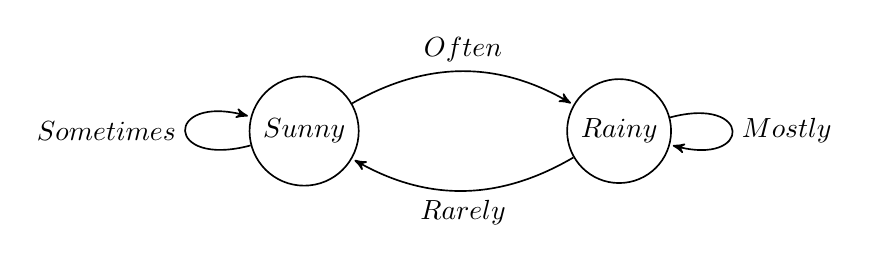
\begin{tikzpicture}[->,>=stealth',shorten >=1pt,auto,node distance=4cm, semithick]   
  \tikzstyle{every state}=[]
  \node[state] (A)              {$Sunny$};   
  \node[state] (B) [right of=A] {$Rainy$};   
  \path (A) edge [loop  left] node {$Sometimes$} (A)
        (A) edge [bend  left] node {    $Often$} (B)
        (B) edge [bend  left] node {   $Rarely$} (A)
        (B) edge [loop right] node {   $Mostly$} (B); 
\end{tikzpicture}

\caption{A two-state Markov chain where the vertices have texts $Sunny$ and
$Rainy$, and the edges have texts $Sometimes$, $Often$, $Rarely$
and $Mostly$\label{fig:named_edges_and_vertices_markov_chain}}
\end{figure}


Here is the code:

\begin{algorithm}[H]
\lstinputlisting[breaklines=true,language={C++}]{create_named_edges_and_vertices_markov_chain.impl}

\caption{Creating the two-state Markov chain as depicted in figure \ref{fig:named_edges_and_vertices_markov_chain}\index{create_named_edges_and_vertices_markov_chain@create\_named\_edges\_and\_vertices\_markov\_chain}\label{alg:create_named_edges_and_vertices_markov_chain}}
\end{algorithm}


Here is the demo:

\begin{algorithm}[H]
\lstinputlisting[breaklines=true,language={C++}]{create_named_edges_and_vertices_markov_chain_demo.impl}

\caption{Demo of the 'create\_named\_edges\_and\_vertices\_markov\_chain' function
(algorithm \ref{alg:create_named_edges_and_vertices_markov_chain})\label{alg:create_named_edges_and_vertices_markov_chain_demo}}
\end{algorithm}



\subsubsection{.dot file}

\begin{algorithm}[H]
\verbatiminput{create_named_edges_and_vertices_markov_chain.dot}

\caption{.dot file created from the 'create\_named\_edges\_and\_vertices\_markov\_chain'
function (algorithm \ref{alg:create_named_edges_and_vertices_markov_chain}),
converted from graph to .dot file using algorithm \ref{alg:save_graph_to_dot}\label{alg:create_named_edges_and_vertices_markov_chain.dot}}
\end{algorithm}



\subsubsection{.svg file}

\begin{figure}[H]
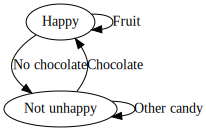
\includegraphics{create_named_edges_and_vertices_markov_chain}

\caption{.svg file created from the 'create\_named\_edges\_and\_vertices\_markov\_chain'
function (algorithm \ref{alg:create_named_edges_and_vertices_markov_chain})
its .dot file, converted from .dot file to .svg using algorithm \ref{alg:convert_dot_to_svg}\label{fig:create_named_edges_and_vertices_markov_chain.svg}}
\end{figure}



\subsection{Creating $K_{3}$ with named edges and vertices\label{sub:create_named_edges_and_vertices_k3}\index{Create $K_{3}$ with named edges and vertices}\index{$K_{3}$ with named edges and vertices, create}}

We extend the graph $K_{2}$ with named vertices of chapter \ref{sub:create_named_vertices_k2_graph}
by adding names to the edges, as depicted in figure \ref{fig:named_edges_and_vertices_k3}:

\begin{figure}[H]
\tikz 
\draw[thick] 
  (2,4) node[fill=black,shape=circle,text=white] {top} 
   -- (3,2) node[anchor=west] {AB} 
   -- (4,0) node[fill=black,shape=circle,text=white] {right} 
   -- (2,0) node[anchor=north] {BC} 
   -- (0,0) node[fill=black,shape=circle,text=white] {left} 
   -- (1,2) node[anchor=east] {CA} 
   -- (2,4)
;

\caption{$K_{3}$: a fully connected graph with three named edges and vertices
\label{fig:named_edges_and_vertices_k3}}
\end{figure}


To create $K_{3}$, the following code can be used:

\begin{algorithm}[H]
\lstinputlisting[breaklines=true,language={C++}]{create_named_edges_and_vertices_k3_graph.impl}

\caption{Creating $K_{3}$ as depicted in figure \ref{fig:named_edges_and_vertices_k3}\index{create_named_edges_and_vertices_k3_graph@create\_named\_edges\_and\_vertices\_k3\_graph}\label{alg:create_named_edges_and_vertices_k3_graph}}
\end{algorithm}


Most of the code is a repeat of algorithm \ref{alg:create_named_vertices_k2_graph}.
In the end, the edge names are obtained as a boost::property\_map
and set. Algorithm \ref{alg:create_named_edges_and_vertices_k3_graph_demo}
shows how to create the graph and measure its edge and vertex names.

\begin{algorithm}[H]
\lstinputlisting[breaklines=true,language={C++}]{create_named_edges_and_vertices_k3_graph_demo.impl}

\caption{Demonstration of the 'create\_named\_edges\_and\_vertices\_k3' function\label{alg:create_named_edges_and_vertices_k3_graph_demo}}
\end{algorithm}



\subsubsection{.dot file\label{sub:create_named_edges_and_vertices_k3_graph.dot}}

\begin{algorithm}[H]
\verbatiminput{create_named_edges_and_vertices_k3_graph.dot}

\caption{.dot file created from the 'create\_named\_edges\_and\_vertices\_k3\_graph'
function (algorithm \ref{alg:create_named_edges_and_vertices_k3_graph}),
converted from graph to .dot file using algorithm \ref{alg:save_graph_to_dot}\label{alg:create_named_edges_and_vertices_k3_graph.dot}}
\end{algorithm}



\subsubsection{.svg file\label{sub:create_named_edges_and_vertices_k3_graph.svg}}

\begin{figure}[H]
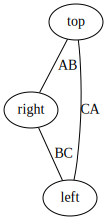
\includegraphics{create_named_edges_and_vertices_k3_graph}

\caption{.svg file created from the 'create\_named\_edges\_and\_vertices\_k3\_graph'
function (algorithm \ref{alg:create_named_edges_and_vertices_k3_graph})
its .dot file, converted from .dot file to .svg using algorithm \ref{alg:convert_dot_to_svg}\label{fig:create_named_edges_and_vertices_k3_graph.svg}}
\end{figure}



\section{Working with graphs with named edges and vertices}

Working with named edges...
\begin{itemize}
\item Check if there exists an edge with a certain name: chapter \ref{sub:has_edge_with_name}
\item Find a (named) edge by its name: chapter \ref{sub:find_first_edge_with_name}
\item Get a (named) edge its name from its edge descriptor: chapter \ref{sub:get_edge_name}
\item Set a (named) edge its name using its edge descriptor: chapter \ref{sub:set_edge_name} 
\item Remove a named edge: chapter \ref{sub:remove_first_edge_with_name}
\item Storing a graph with named edges and vertices as a .dot file: chapter
\ref{sub:save_named_edges_and_vertices_undirected_graph_to_dot}
\item Loading a graph with named edges and vertices from a .dot file: chapter 
\end{itemize}
Especially chapter \ref{sub:find_first_edge_with_name} with the 'find\_first\_edge\_by\_name'
algorithm shows how to obtain an edge descriptor, which is used in
later algorithms.


\subsection{Check if there exists an edge with a certain name\label{sub:has_edge_with_name}}

Before modifying our edges, let's first determine if we can find an
edge by its name in a graph. After obtaing a name map, we obtain the
edge iterators, dereference these to obtain the edge descriptors and
then compare each edge its name with the one desired.

\begin{algorithm}[H]
\lstinputlisting[breaklines=true,language={C++}]{has_edge_with_name.impl}

\caption{Find if there is an edge with a certain name\index{has_edge_with_name@has\_edge\_with\_name}\label{alg:has_edge_with_name}}
\end{algorithm}


This function can be demonstrated as in algorithm \ref{alg:has_edge_with_name_demo},
where a certain name cannot be found in an empty graph. After adding
the desired name, it is found.

\begin{algorithm}[H]
\lstinputlisting[breaklines=true,language={C++}]{has_edge_with_name_demo.impl}

\caption{Demonstration of the 'has\_edge\_with\_name' function\label{alg:has_edge_with_name_demo}}
\end{algorithm}


Note that this function only finds if there is at least one edge with
that name: it does not tell how many edges with that name exist in
the graph.


\subsection{Find an edge by its name\label{sub:find_first_edge_with_name}}

Where STL functions work with iterators, here we obtain an edge descriptor
(see chapter \ref{sub:Edge-descriptors}) to obtain a handle to the
desired edge. Algorithm \ref{alg:find_first_edge_with_name} shows
how to obtain an edge descriptor to the first (name) edge found with
a specific name.

\begin{algorithm}[H]
\lstinputlisting[breaklines=true,language={C++}]{find_first_edge_with_name.impl}

\caption{Find the first edge by its name\index{find_first_edge_by_name@find\_first\_edge\_by\_name}\label{alg:find_first_edge_with_name}}
\end{algorithm}


With the edge descriptor obtained, one can read and modify the graph.
Algorithm \ref{alg:find_first_edge_with_name_demo} shows some examples
of how to do so.

\begin{algorithm}[H]
\lstinputlisting[breaklines=true,language={C++}]{find_first_edge_with_name_demo.impl}

\caption{Demonstration of the 'find\_first\_edge\_by\_name' function\label{alg:find_first_edge_with_name_demo}}
\end{algorithm}



\subsection{Get a (named) edge its name from its edge descriptor\label{sub:get_edge_name}}

This may seem a trivial paragraph, as chapter \ref{sub:get_edge_names}
describes the 'get\_edge\_names' algorithm, in which we get all edges'
names. But it does not allow to first find an edge of interest and
subsequently getting only that one its name.

To obtain the name from an edgedescriptor, one needs to pull out the
name map and then look up the edge of interest.

\begin{algorithm}[H]
\lstinputlisting[breaklines=true,language={C++}]{get_edge_name.impl}

\caption{Get an edge its name from its edge descriptor\index{get_edge_name@get\_edge\_name}\label{alg:get_edge_name}}
\end{algorithm}


To use 'get\_edge\_name', one first needs to obtain an edge descriptor.
Algorithm \ref{alg:get_edge_name_demo} shows a simple example.

\begin{algorithm}[H]
\lstinputlisting[breaklines=true,language={C++}]{get_edge_name_demo.impl}

\caption{Demonstration if the 'get\_edge\_name' function\label{alg:get_edge_name_demo}}
\end{algorithm}



\subsection{Set a (named) edge its name from its edge descriptor\label{sub:set_edge_name}}

If you know how to get the name from an edge descriptor, setting it
is just as easy, as shown in algorithm \ref{alg:set_edge_name}.

\begin{algorithm}[H]
\lstinputlisting[breaklines=true,language={C++}]{set_edge_name.impl}

\caption{Set an edge its name from its edge descriptor\index{set_edge_name@set\_edge\_name}\label{alg:set_edge_name}}
\end{algorithm}


To use 'set\_edge\_name', one first needs to obtain an edge descriptor.
Algorithm \ref{alg:set_edge_name_demo} shows a simple example.

\begin{algorithm}[H]
\lstinputlisting[breaklines=true,language={C++}]{set_edge_name_demo.impl}

\caption{Demonstration if the 'set\_edge\_name' function\label{alg:set_edge_name_demo}}
\end{algorithm}



\subsection{Removing the first edge with a certain name\label{sub:remove_first_edge_with_name}}

An edge descriptor can be used to remove an edge from a graph. 

Removing a named edge goes as follows: use the name of the edge to
get a first edge descriptor, then call 'boost::remove\_edge'\index{boost::remove_edge@boost::remove\_edge},
shown in algorithm \ref{alg:remove_first_vertex_with_name}:

\begin{algorithm}[H]
\lstinputlisting[breaklines=true,language={C++}]{remove_first_edge_with_name.impl}

\caption{Remove the first edge with a certain name\index{remove_first_edge_with_name@remove\_first\_edge\_with\_name}\label{alg:remove_first_edge_with_name}}
\end{algorithm}


Algorithm \ref{alg:remove_first_edge_with_name_demo} shows the removal
of the first named edge found.

\begin{algorithm}[H]
\lstinputlisting[breaklines=true,language={C++}]{remove_first_edge_with_name_demo.impl}

\caption{Demonstration of the 'remove\_first\_edge\_with\_name' function\label{alg:remove_first_edge_with_name_demo}}
\end{algorithm}



\subsection{Storing an undirected graph with named edges and vertices as a .dot\label{sub:save_named_edges_and_vertices_undirected_graph_to_dot}\index{Save graph with name edges and vertices as .dot}\index{Create .dot from graph with named edges and vertices}}

If you used the create\_named\_edges\_and\_vertices\_k3\_graph function
(algorithm \ref{alg:create_named_edges_and_vertices_k3_graph}) to
produce a $K_{3}$ graph with named edges and vertices, you can store
these names additionally with algorithm \ref{alg:save_named_edges_and_vertices_graph_to_dot}:

\begin{algorithm}[H]
\lstinputlisting[breaklines=true,language={C++}]{save_named_edges_and_vertices_graph_to_dot_cpp17.impl}

\caption{Storing a graph with named edges and vertices as a .dot file\index{save_named_edges_and_vertices_graph_to_dot@save\_named\_edges\_and\_vertices\_graph\_to\_dot}\label{alg:save_named_edges_and_vertices_graph_to_dot}}
\end{algorithm}


Note that this algorithm uses C++17\index{C++17}.

The .dot file created is displayed in algorithm \ref{alg:save_named_edges_and_vertices_graph_to_dot_test_named_vertices_k3_graph.dot}:

\begin{algorithm}[H]
\verbatiminput{save_named_edges_and_vertices_graph_to_dot_test_named_edges_and_vertices_k3_graph.dot}

\caption{.dot file created from the create\_named\_edges\_and\_vertices\_k3\_graph
function (algorithm \ref{alg:create_named_vertices_k2_graph})\label{alg:save_named_edges_and_vertices_graph_to_dot_test_named_vertices_k3_graph.dot}}
\end{algorithm}


This .dot file corresponds to figure \ref{fig:save_named_edges_and_vertices_graph_to_dot_test_named_vertices_k2_graph.svg}:

\begin{figure}[H]
\includegraphics{save_named_edges_and_vertices_graph_to_dot_test_named_edges_and_vertices_k3_graph}

\caption{.svg file created from the create\_named\_edges\_and\_vertices\_k3\_graph
function (algorithm \ref{alg:create_named_vertices_k2_graph}) and
converted to .svg using the 'convert\_dot\_to\_svg' function (algorithm
\ref{alg:convert_dot_to_svg})\label{fig:save_named_edges_and_vertices_graph_to_dot_test_named_vertices_k2_graph.svg}}
\end{figure}


If you created a graph with edges more complex than just a name, you
will still just write these to the .dot file. Chapter \ref{sub:save_custom_vertices_graph_to_dot}
shows how to write custom vertices to a .dot file.

So, the 'save\_named\_edges\_and\_vertices\_graph\_to\_dot' function
(algorithm \ref{alg:save_graph_to_dot}) saves only the structure
of the graph and its edge and vertex names.


\subsection{Loading a directed graph with named edges and vertices from a .dot\label{sub:load_directed_named_edges_and_vertices_graph_from_dot}\index{Load directed graph with named edges and vertices from .dot}\index{Create directed graph with named edges and vertices from .dot} }

When loading a graph from file, one needs to specify a type of graph.
In this example, an directed graph with named edges and vertices is
loaded, as shown in algorithm \ref{alg:load_directed_named_edges_and_vertices_graph_from_dot}:

\begin{algorithm}[H]
\lstinputlisting[breaklines=true,language={C++}]{load_directed_named_edges_and_vertices_graph_from_dot.impl}

\caption{Loading a directed graph with named edges and vertices from a .dot
file\index{load_directed_named_edges_and_vertices_graph_from_dot@load\_directed\_named\_edges\_and\_vertices\_graph\_from\_dot}\label{alg:load_directed_named_edges_and_vertices_graph_from_dot}}
\end{algorithm}


In this algorithm, first it is checked if the file to load exists.
Then an empty directed graph is created. Next to this, a boost::dynamic\_properties\index{boost::dynamic_properties@boost::dynamic\_properties}
is created with its default constructor, after which we direct the
boost::dynamic\_properties\index{boost::dynamic_properties@boost::dynamic\_properties}
to find a 'node\_id' and 'label' in the vertex name map, 'edge\_id'
and 'label to the edge name map. From this and the empty graph, 'boost::read\_graphviz'\index{boost::read_graphviz@boost::read\_graphviz}
is called to build up the graph.

Algorithm \ref{alg:load_directed_named_edges_and_vertices_graph_from_dot_demo}
shows how to use the 'load\_directed\_graph\_from\_dot' function:

\begin{algorithm}[H]
\lstinputlisting[breaklines=true,language={C++}]{load_directed_named_edges_and_vertices_graph_from_dot_demo.impl}

\caption{Demonstration of the 'load\_directed\_named\_edges\_and\_vertices\_graph\_from\_dot'
function\label{alg:load_directed_named_edges_and_vertices_graph_from_dot_demo}}
\end{algorithm}


This demonstration shows how the Markov chain is created using the
'create\_named\_edges\_and\_vertices\_markov\_chain' function (algorithm
\ref{alg:create_named_edges_and_vertices_markov_chain}), saved and
then loaded. The loaded graph is checked to be a directed graph similar
to the Markov chain with the same edge and vertex names (using the
'get\_edge\_names' function , algorithm \ref{alg:get_edge_names},
and the 'get\_vertex\_names' function, algorithm \ref{alg:get_vertex_names}).


\subsection{Loading an undirected graph with named edges and vertices from a
.dot\label{sub:load_undirected_named_edges_and_vertices_graph_from_dot}\index{Load undirected graph with named edges and vertices from .dot}\index{Create undirected graph with named edges and vertices from .dot}}

When loading a graph from file, one needs to specify a type of graph.
In this example, an undirected graph with named edges and vertices
is loaded, as shown in algorithm \ref{alg:load_undirected_named_edges_and_vertices_graph_from_dot}:

\begin{algorithm}[H]
\lstinputlisting[breaklines=true,language={C++}]{load_undirected_named_edges_and_vertices_graph_from_dot.impl}

\caption{Loading an undirected graph with named edges and vertices from a .dot
file\index{load_undirected_named_edges_and_vertices_graph_from_dot@load\_undirected\_named\_edges\_and\_vertices\_graph\_from\_dot}\label{alg:load_undirected_named_edges_and_vertices_graph_from_dot}}
\end{algorithm}


In this algorithm, first it is checked if the file to load exists.
Then an empty directed graph is created. Next to this, a boost::dynamic\_properties\index{boost::dynamic_properties@boost::dynamic\_properties}
is created with its default constructor, after which we direct the
boost::dynamic\_properties\index{boost::dynamic_properties@boost::dynamic\_properties}
to find a 'node\_id' and 'label' in the vertex name map, 'edge\_id'
and 'label to the edge name map. From this and the empty graph, 'boost::read\_graphviz'\index{boost::read_graphviz@boost::read\_graphviz}
is called to build up the graph.

Algorithm \ref{alg:load_undirected_named_edges_and_vertices_graph_from_dot_demo}
shows how to use the 'load\_undirected\_graph\_from\_dot' function:

\begin{algorithm}[H]
\lstinputlisting[breaklines=true,language={C++}]{load_undirected_named_edges_and_vertices_graph_from_dot_demo.impl}

\caption{Demonstration of the 'load\_undirected\_named\_edges\_and\_vertices\_graph\_from\_dot'
function\label{alg:load_undirected_named_edges_and_vertices_graph_from_dot_demo}}
\end{algorithm}


This demonstration shows how $K_{3}$ with named edges and vertices
is created using the 'create\_named\_edges\_and\_vertices\_k3\_graph'
function (algorithm \ref{alg:create_named_edges_and_vertices_k3_graph}),
saved and then loaded. The loaded graph is checked to be an undirected
graph similar to $K_{3}$ , with the same edge and vertex names (using
the 'get\_edge\_names' function , algorithm \ref{alg:get_edge_names},
and the 'get\_vertex\_names' function, algorithm \ref{alg:get_vertex_names}).


\section{Building graphs with custom vertices}

Up until now, the graphs created have had edges and vertices with
the built-in name propery. In this chapter, graphs will be created,
in which the vertices can have a custom 'my\_vertex' type%
\footnote{I do not intend to be original in naming my data types%
}. The following graphs will be created:
\begin{itemize}
\item An empty directed graph that allows for custom vertices: see chapter
\ref{alg:create_empty_directed_custom_vertices_graph}
\item An empty undirected graph that allows for custom vertices: see chapter 
\item A two-state Markov chain with custom vertices: see chapter 
\item $K_{2}$with custom vertices: see chapter \ref{sub:create_custom_vertices_k2_graph}
\end{itemize}
In the process, some basic (sometimes bordering trivial) functions
are shown:
\begin{itemize}
\item Create the custom vertex class, called 'my\_vertex'
\item Installing the new vertex type as a vertex property, called 'vertex\_custom\_type\index{vertex_custom_type@vertex\_custom\_type}'
\item Adding a custom vertex: see chapter \ref{sub:add_custom_vertex}
\end{itemize}
Additionally, will will need to:

These functions are mostly there for completion and showing which
data types are used.


\subsection{Creating the custom vertex class\label{sub:my_vertex}}

Before creating an empty graph with custom vertices, that custom vertex
class must be created. Here I will show the header file of it, as
the implementation of it is not important yet.

\begin{algorithm}[H]
\lstinputlisting[breaklines=true,language={C++}]{my_vertex.h}

\caption{Declaration of my\_vertex\index{my_vertex@my\_vertex}\index{my_vertex.h@my\_vertex.h}\index{my_vertex declaration@my\_vertex declaration}\index{Declaration, my_vertex@Declaration, my\_vertex}\label{alg:my_vertex_h}}
\end{algorithm}


my\_vertex is a class that has multiple properties: two doubles 'm\_x'
('m\_\index{m_@m\_}' stands for member\index{member}) and 'm\_y',
and two std::strings m\_name and m\_description. my\_vertex is copyable,
but cannot trivially be converted to a std::string.


\subsection{Installing the new vertex property\label{sub:install_vertex_custom_type}}

Before creating an empty graph with custom vertices, this type must
be installed as a vertex property. Installing a new property would
have been easier, if 'more C++ compilers were standards conformant'
(\cite{siek2001boost} chapter 3.6). Boost.Graph uses the BOOST\_INSTALL\_PROPERTY\index{BOOST_INSTALL_PROPERTY@BOOST\_INSTALL\_PROPERTY}
macro\index{macro} to allow using a custom property:

\begin{algorithm}[H]
\lstinputlisting[breaklines=true,language={C++}]{install_vertex_custom_type.impl}

\caption{Installing the vertex\_custom\_type property\index{install_vertex_custom_type@install\_vertex\_custom\_type}\label{alg:install_vertex_custom_type}}
\end{algorithm}


The enum value 314 must be unique.


\subsection{Create the empty directed graph with custom vertices\label{sub:create_empty_directed_custom_vertices_graph}}

\begin{algorithm}[H]
\lstinputlisting[breaklines=true,language={C++}]{create_empty_directed_custom_vertices_graph.impl}

\caption{Creating an empty directed graph with custom vertices\index{create_empty_directed_custom_vertices_graph@create\_empty\_directed\_custom\_vertices\_graph}\label{alg:create_empty_directed_custom_vertices_graph}}
\end{algorithm}


This graph:
\begin{itemize}
\item has its out edges stored in a std::vector (due to the first boost::vecS\index{boost::vecS})
\item has its vertices stored in a std::vector (due to the second boost::vecS\index{boost::vecS})
\item is directed (due to the boost::directedS\index{boost::directedS})
\item The vertices have one property: they have a custom type, that is of
data type my\_vertex (due to the boost::property< boost::vertex\_custom\_type\_t,my\_vertex>\index{boost::property}\index{boost::vertex_custom_type_t@boost::vertex\_custom\_type\_t}\index{my_vertex@my\_vertex}')
\item The edges and graph have no properties
\item Edges are stored in a std::list
\end{itemize}
The boost::adjacency\_list\index{boost::adjacency_list@boost::adjacency\_list}
has a new, fourth template argument 'boost::property< boost::vertex\_custom\_type\_t,my\_vertex>\index{boost::property}\index{boost::vertex_custom_type_t@boost::vertex\_custom\_type\_t}\index{my_vertex@my\_vertex}'.
This can be read as: ``vertices have the property 'boost::vertex\_custom\_type\_t',
which is of data type 'my\_vertex'''. Or simply: ``vertices have
a custom type called my\_vertex''.


\subsection{Create the empty undirected graph with custom vertices\label{sub:create_empty_undirected_custom_vertices_graph}}

\begin{algorithm}[H]
\lstinputlisting[breaklines=true,language={C++}]{create_empty_undirected_custom_vertices_graph.impl}

\caption{Creating an empty undirected graph with custom vertices\index{create_empty_undirected_custom_vertices_graph@create\_empty\_undirected\_custom\_vertices\_graph}\label{alg:create_empty_undirected_custom_vertices_graph}}
\end{algorithm}


This graph:
\begin{itemize}
\item has its out edges stored in a std::vector (due to the first boost::vecS\index{boost::vecS})
\item has its vertices stored in a std::vector (due to the second boost::vecS\index{boost::vecS})
\item is undirected (due to the boost::undirectedS\index{boost::undirectedS})
\item The vertices have one property: they have a custom type, that is of
data type my\_vertex (due to the boost::property< boost::vertex\_custom\_type\_t,my\_vertex>\index{boost::property}\index{boost::vertex_custom_type_t@boost::vertex\_custom\_type\_t}\index{my_vertex@my\_vertex}')
\item The edges and graph have no properties
\item Edges are stored in a std::list
\end{itemize}
The boost::adjacency\_list\index{boost::adjacency_list@boost::adjacency\_list}
has a new, fourth template argument 'boost::property< boost::vertex\_custom\_type\_t,my\_vertex>\index{boost::property}\index{boost::vertex_custom_type_t@boost::vertex\_custom\_type\_t}\index{my_vertex@my\_vertex}'.
This can be read as: ``vertices have the property 'boost::vertex\_custom\_type\_t',
which is of data type 'my\_vertex'''. Or simply: ``vertices have
a custom type called my\_vertex''.


\subsection{Add a custom vertex\label{sub:add_custom_vertex}}

Adding a custom vertex is very similar to adding a named vertex (chapter
\ref{sub:add_named_vertex}).

\begin{algorithm}[H]
\lstinputlisting[breaklines=true,language={C++}]{add_custom_vertex.impl}

\caption{Add a custom vertex\index{add_custom_vertex@add\_custom\_vertex}\label{alg:add_custom_vertex}}
\end{algorithm}


When having added a new (abstract) vertex to the graph, the vertex
descriptor is used to set the my\_vertex in the graph its my\_vertex
map (using 'get(boost::vertex\_custom\_type,g)\index{boost::vertex_custom_type@boost::vertex\_custom\_type}\index{get}').


\subsection{Getting the vertices' my\_vertexes%
\footnote{the name 'my\_vertexes' is chosen to indicate this function returns
a container of my\_vertex%
}\label{sub:get_vertex_my_vertexes}}

When the vertices of a graph have any associated my\_vertex, one can
extract these as such:

\begin{algorithm}[H]
\lstinputlisting[breaklines=true,language={C++}]{get_vertex_my_vertexes.impl}

\caption{Get the vertices' my\_vertexes\index{get_vertex_my_vertexes@get\_vertex\_my\_vertexes}\label{alg:get_vertex_my_vertexes}}
\end{algorithm}


The my\_vertex object associated with the vertices are obtained from
a boost::property\_map and then put into a std::vector.

When trying to get the vertices' my\_vertex from a graph without my\_vertex
objects associated, you will get the error 'formed reference to void'
(see chapter \ref{sub:formed_reference_to_void}).


\subsection{Creating a two-state Markov chain with custom vertices\label{sub:create_custom_vertices_markov_chain}}

We build this graph:

\begin{figure}[H]
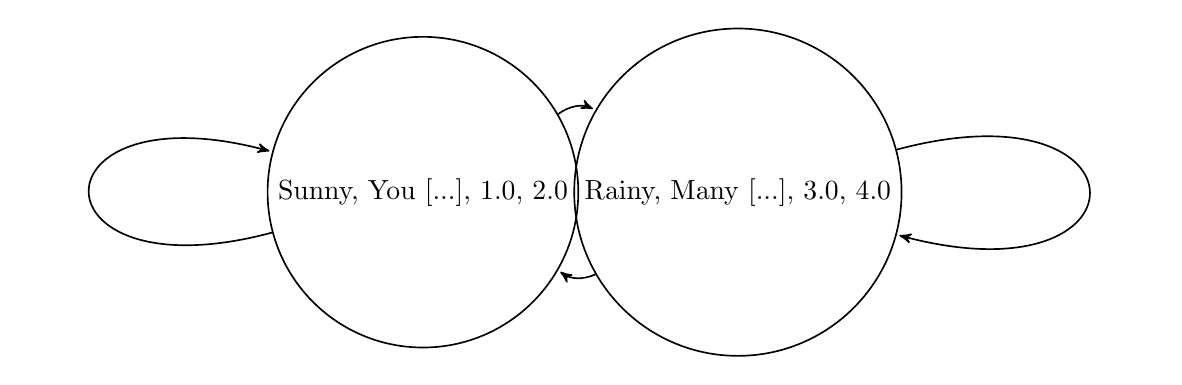
\begin{tikzpicture}[->,>=stealth',shorten >=1pt,auto,node distance=4cm, semithick]   
  \tikzstyle{every state}=[]
  \node[state] (A) 
    {Sunny, You [...], 1.0, 2.0};   
  \node[state] (B) [right of=A] 
    {Rainy, Many [...], 3.0, 4.0}
  ;   
  \path (A) edge [loop  left] node {} (A)
        (A) edge [bend  left] node {} (B)
        (B) edge [bend  left] node {} (A)
        (B) edge [loop right] node {} (B); 
\end{tikzpicture}

\caption{A two-state Markov chain where the vertices have custom properies
and the edges have no properties. The left vertex has (1) the text
$Sunny$ , (2) the description 'You can see the yellow thing' (which
is abbreviated), (3) an $x$ of $1.0$, and, (4) a $y$ of $2.0$.
The right vertex has (1) the text $Rainy$ , (2) the description 'Many
grey fluffy things' (which is abbreviated), (3) an $x$ of $3.0$,
and, (4) a $y$ of $4.0$. The text is abbreviated to get a nicer
figure. The vertices' properties are nonsensical\label{fig:custom_vertices_markov_chain}}
\end{figure}


Here is the code:

\begin{algorithm}[H]
\lstinputlisting[breaklines=true,language={C++}]{create_custom_vertices_markov_chain.impl}

\caption{Creating the two-state Markov chain as depicted in figure \ref{fig:custom_vertices_markov_chain}\index{create_custom_vertices_markov_chain@create\_custom\_vertices\_markov\_chain}\label{alg:create_custom_vertices_markov_chain}}
\end{algorithm}


Here is the demo:

\begin{algorithm}[H]
\lstinputlisting[breaklines=true,language={C++}]{create_custom_vertices_markov_chain_demo.impl}

\caption{Demo of the 'create\_custom\_vertices\_markov\_chain' function (algorithm
\ref{alg:create_custom_vertices_markov_chain})\label{alg:create_custom_and_vertices_markov_chain_demo}}
\end{algorithm}



\subsubsection{.dot file}

\begin{algorithm}[H]
\verbatiminput{create_custom_vertices_markov_chain.dot}

\caption{.dot file created from the 'create\_custom\_vertices\_markov\_chain'
function (algorithm \ref{alg:create_custom_vertices_markov_chain}),
converted from graph to .dot file using algorithm \ref{alg:save_graph_to_dot}\label{alg:create_custom_vertices_markov_chain.dot}}
\end{algorithm}



\subsubsection{.svg file}

\begin{figure}[H]
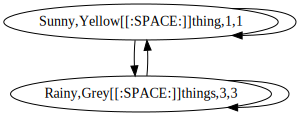
\includegraphics{create_custom_vertices_markov_chain}

\caption{.svg file created from the 'create\_custom\_vertices\_markov\_chain'
function (algorithm \ref{alg:create_custom_vertices_markov_chain})
its .dot file, converted from .dot file to .svg using algorithm \ref{alg:convert_dot_to_svg}\label{fig:create_custom_vertices_markov_chain.svg}}
\end{figure}



\subsection{Creating $K_{2}$ with custom vertices\label{sub:create_custom_vertices_k2_graph}}

We reproduce the $K_{2}$ with named vertices of chapter \ref{sub:create_named_vertices_k2_graph}
, but with our custom vertices intead:

\begin{algorithm}[H]
\lstinputlisting[breaklines=true,language={C++}]{create_custom_vertices_k2_graph.impl}

\caption{Creating $K_{2}$ as depicted in figure \ref{fig:named_vertices_k2_graph}\index{create_custom_vertices_k2_graph@create\_custom\_vertices\_k2\_graph}\label{alg:create_custom_vertices_k2_graph}}
\end{algorithm}


Most of the code is a slight modification of the 'create\_named\_vertices\_k2\_graph'
function (algorithm \ref{alg:create_named_vertices_k2_graph}). In
the end, the my\_vertices are obtained as a boost::property\_map and
set with two custom my\_vertex objects.

Demo:

\begin{algorithm}[H]
\lstinputlisting[breaklines=true,language={C++}]{create_custom_vertices_k2_graph_demo.impl}

\caption{Demo of the 'create\_custom\_vertices\_k2\_graph' function (algorithm
\ref{alg:create_custom_vertices_k2_graph})\label{alg:create_custom_and_vertices_k2_graph_demo}}
\end{algorithm}



\subsubsection{.dot file}

\begin{algorithm}[H]
\verbatiminput{create_custom_vertices_k2_graph.dot}

\caption{.dot file created from the 'create\_custom\_vertices\_k2\_graph' function
(algorithm \ref{alg:create_custom_vertices_k2_graph}), converted
from graph to .dot file using algorithm \ref{alg:save_graph_to_dot}\label{alg:create_custom_vertices_k2_graph.dot}}
\end{algorithm}



\subsubsection{.svg file}

\begin{figure}[H]
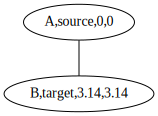
\includegraphics{create_custom_vertices_k2_graph}

\caption{.svg file created from the 'create\_custom\_vertices\_k2\_graph' function
(algorithm \ref{alg:create_custom_vertices_k2_graph}) its .dot file,
converted from .dot file to .svg using algorithm \ref{alg:convert_dot_to_svg}\label{fig:create_custom_vertices_k2_graph.svg}}
\end{figure}



\section{Measuring simple graphs traits of a graph with custom vertices}


\subsection{Has a my\_vertex\label{sub:has_vertex_with_my_vertex}}

Before modifying our vertices, let's first determine if we can find
a vertex by its custom type ('my\_vertex') in a graph. After obtaing
a my\_vertex map, we obtain the vertex iterators, dereference these
to obtain the vertex descriptors and then compare each vertex its
my\_vertex with the one desired.

\begin{algorithm}[H]
\lstinputlisting[breaklines=true,language={C++}]{has_vertex_with_my_vertex.impl}

\caption{Find if there is vertex with a certain my\_vertex\index{has_vertex_with_my_vertex@has\_vertex\_with\_my\_vertex}\label{alg:has_vertex_with_my_vertex}}
\end{algorithm}


This function can be demonstrated as in algorithm \ref{alg:has_vertex_with_my_vertex_demo},
where a certain my\_vertex cannot be found in an empty graph. After
adding the desired my\_vertex, it is found.

\begin{algorithm}[H]
\lstinputlisting[breaklines=true,language={C++}]{has_vertex_with_my_vertex_demo.impl}

\caption{Demonstration of the 'has\_vertex\_with\_my\_vertex' function\label{alg:has_vertex_with_my_vertex_demo}}
\end{algorithm}


Note that this function only finds if there is at least one vertex
with that my\_vertex: it does not tell how many vertices with that
my\_vertex exist in the graph.


\subsection{Find a vertex with a certain my\_vertex\label{sub:find_vertex_with_my_vertex}}

Where STL functions work with iterators, here we obtain a vertex descriptor
(see chapter \ref{sub:Vertex-descriptors}) to obtain a handle to
the desired vertex. Algorithm \ref{alg:find_first_vertex_with_my_vertex}
shows how to obtain a vertex descriptor to the first vertex found
with a specific my\_vertex value.

\begin{algorithm}[H]
\lstinputlisting[breaklines=true,language={C++}]{find_first_vertex_with_my_vertex.impl}

\caption{Find the first vertex with a certain my\_vertex\index{find_first_vertex_with_my_vertex@find\_first\_vertex\_with\_my\_vertex}\label{alg:find_first_vertex_with_my_vertex}}
\end{algorithm}


With the vertex descriptor obtained, one can read and modify the vertex
and the edges surrounding it. Algorithm \ref{alg:find_first_vertex_with_my_vertex_demo}
shows some examples of how to do so.

\begin{algorithm}[H]
\lstinputlisting[breaklines=true,language={C++}]{find_first_vertex_with_my_vertex_demo.impl}

\caption{Demonstration of the 'find\_first\_vertex\_with\_my\_vertex' function\label{alg:find_first_vertex_with_my_vertex_demo}}
\end{algorithm}



\subsection{Get a vertex its my\_vertex\label{sub:get_vertex_my_vertex}}

To obtain the name from a vertex descriptor, one needs to pull out
the my\_vertexes%
\footnote{Bad English intended: my\_vertexes = multiple my\_vertex objects,
vertices = multiple graph nodes%
} map and then look up the vertex of interest.

\begin{algorithm}[H]
\lstinputlisting[breaklines=true,language={C++}]{get_vertex_my_vertex.impl}

\caption{Get a vertex its my\_vertex from its vertex descriptor\index{get_vertex_my_vertex@get\_vertex\_my\_vertex}\label{alg:get_vertex_my_vertex}}
\end{algorithm}


To use 'get\_vertex\_my\_vertex', one first needs to obtain a vertex
descriptor. Algorithm \ref{alg:get_vertex_my_vertex_demo} shows a
simple example.

\begin{algorithm}[H]
\lstinputlisting[breaklines=true,language={C++}]{get_vertex_my_vertex_demo.impl}

\caption{Demonstration if the 'get\_vertex\_my\_vertex' function\label{alg:get_vertex_my_vertex_demo}}
\end{algorithm}



\subsection{Set a vertex its my\_vertex\label{sub:set_vertex_my_vertex}}

If you know how to get the my\_vertex from a vertex descriptor, setting
it is just as easy, as shown in algorithm \ref{alg:set_vertex_my_vertex}.

\begin{algorithm}[H]
\lstinputlisting[breaklines=true,language={C++}]{set_vertex_my_vertex.impl}

\caption{Set a vertex its my\_vertex from its vertex descriptor\index{set_vertex_my_vertex@set\_vertex\_my\_vertex}\label{alg:set_vertex_my_vertex}}
\end{algorithm}


To use 'set\_vertex\_my\_vertex', one first needs to obtain a vertex
descriptor. Algorithm \ref{alg:set_vertex_my_vertex_demo} shows a
simple example.

\begin{algorithm}[H]
\lstinputlisting[breaklines=true,language={C++}]{set_vertex_my_vertex_demo.impl}

\caption{Demonstration if the 'set\_vertex\_my\_vertex' function\label{alg:set_vertex_my_vertex_demo}}
\end{algorithm}



\subsection{Setting all vertices' my\_vertex objects\label{sub:set_vertex_my_vertexes}\index{Set vertices my_vertexes@Set vertices my\_vertexes}\index{Vertices, set my_vertexes@Vertices, set my\_vertexes}}

When the vertices of a graph are associated with my\_vertex objects,
one can set these my\_vertexes as such:

\begin{algorithm}[H]
\lstinputlisting[breaklines=true,language={C++}]{set_vertex_my_vertexes.impl}

\caption{Setting the vertices' my\_vertexes\index{set_vertex_my_vertexes@set\_vertex\_my\_vertexes}\label{alg:set_vertex_my_vertexes}}
\end{algorithm}


An impressive feature is that getting the property map holding the
graph its names is not a copy, but a reference. Otherwise, modifying
'my\_vertexes\_map' (obtained by non-reference) would only modify
a copy.


\subsection{Storing a graph with custom vertices as a .dot\label{sub:save_custom_vertices_graph_to_dot}\index{Save graph with custom vertices as .dot}\index{Create .dot from graph with custom vertices} }

If you used the create\_custom\_vertices\_k2\_graph function (algorithm
\ref{alg:create_custom_vertices_k2_graph}) to produce a $K_{2}$
graph with vertices associated with my\_vertex objects, you can store
these my\_vertexes additionally with algorithm \ref{alg:save_custom_vertices_graph_to_dot}:

\begin{algorithm}[H]
\lstinputlisting[breaklines=true,language={C++}]{save_custom_vertices_graph_to_dot_cpp14.impl}

\caption{Storing a graph with custom vertices as a .dot file\index{save_custom_vertices_graph_to_dot@save\_custom\_vertices\_graph\_to\_dot}\label{alg:save_custom_vertices_graph_to_dot}}
\end{algorithm}


Note that this algorithm uses C++14\index{C++14}.

The .dot file created is displayed in algorithm \ref{alg:save_custom_vertices_graph_to_dot_test_custom_vertices_k2_graph.dot}:

\begin{algorithm}[H]
\verbatiminput{save_custom_vertices_graph_to_dot_test_custom_vertices_k2_graph.dot}

\caption{.dot file created from the create\_custom\_vertices\_k2\_graph function
(algorithm \ref{alg:create_named_vertices_k2_graph})\label{alg:save_custom_vertices_graph_to_dot_test_custom_vertices_k2_graph.dot}}
\end{algorithm}


This .dot file corresponds to figure \ref{alg:save_custom_vertices_graph_to_dot_test_custom_vertices_k2_graph.dot}:

\begin{figure}[H]
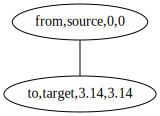
\includegraphics{save_custom_vertices_graph_to_dot_test_custom_vertices_k2_graph}

\caption{.svg file created from the create\_custom\_vertices\_k2\_graph function
(algorithm \ref{alg:create_custom_vertices_k2_graph}) and converted
to .svg using the 'convert\_dot\_to\_svg' function (algorithm \ref{alg:convert_dot_to_svg})\label{fig:save_custom_vertices_graph_to_dot_test_custom_vertices_k2_graph.svg}}
\end{figure}



\section{Building graphs with custom edges and vertices}

Up until now, the graphs created have had edges and vertices with
the built-in name propery. In this chapter, graphs will be created,
in which the edges and vertices can have a custom 'my\_edge' and 'my\_edge'
type%
\footnote{I do not intend to be original in naming my data types%
}.
\begin{itemize}
\item An empty (undirected) graph that allows for custom edges and vertices:
see chapter \ref{sub:create_empty_custom_edges_and_vertices_graph}
\item $K_{3}$with custom edges and vertices: see chapter \ref{sub:create_custom_edges_and_vertices_k3}
\end{itemize}
In the process, some basic (sometimes bordering trivial) functions
are shown:
\begin{itemize}
\item Adding a custom edge: see chapter \ref{sub:add_custom_edge}
\end{itemize}
These functions are mostly there for completion and showing which
data types are used.


\subsection{Create an empty graph with custom edges and vertices\label{sub:create_empty_custom_edges_and_vertices_graph}}

Say we want to use our own edge class as graph nodes. This is done
in multiple steps:
\begin{enumerate}
\item Create a custom edge class, called 'my\_edge'
\item Install a new property, called 'edge\_custom\_type\index{edge_custom_type@edge\_custom\_type}'
\item Use the new property in creating a boost::adjacency\_list
\end{enumerate}

\subsubsection{Creating the custom edge class}

In this example, I create a custom edge class. Here I will show the
header file of it, as the implementation of it is not important yet.

\begin{algorithm}[H]
\lstinputlisting[breaklines=true,language={C++}]{my_edge.h}

\caption{Declaration of my\_edge\index{my_edge@my\_edge}\index{my_edge.h@my\_edge.h}\index{my_edge declaration@my\_edge declaration}\index{Declaration, my_edge@Declaration, my\_edge}\label{alg:my_edge_h}}
\end{algorithm}


my\_edge is a class that has multiple properties: two doubles 'm\_width'
('m\_\index{m_@m\_}' stands for member\index{member}) and 'm\_height',
and two std::strings m\_name and m\_description. my\_edge is copyable,
but cannot trivially be converted to a std::string.


\subsubsection{Installing the new property}

Installing a new property would have been easier, if 'more C++ compilers
were standards conformant' (\cite{siek2001boost}, chapter 3.6, footnote
at page 52). Boost.Graph uses the BOOST\_INSTALL\_PROPERTY\index{BOOST_INSTALL_PROPERTY@BOOST\_INSTALL\_PROPERTY}
macro\index{macro} to allow using a custom property:

\begin{algorithm}[H]
\lstinputlisting[breaklines=true,language={C++}]{install_edge_custom_type.impl}

\caption{Installing the edge\_custom\_type property\index{install_vertex_custom_type@install\_vertex\_custom\_type}\label{alg:install_edge_custom_type}}
\end{algorithm}


The enum value 3142\index{pi} must be unique.


\subsubsection{Create the empty undirected graph with custom edges and vertices}

\begin{algorithm}[H]
\lstinputlisting[breaklines=true,language={C++}]{create_empty_undirected_custom_edges_and_vertices_graph.impl}

\caption{Creating an empty undirected graph with custom edges and vertices\index{create_empty_undirected_custom_vertices_graph@create\_empty\_undirected\_custom\_vertices\_graph}\label{alg:create_empty_undirected_custom_edges_and_vertices_graph}}
\end{algorithm}


This graph:
\begin{itemize}
\item has its out edges stored in a std::vector (due to the first boost::vecS\index{boost::vecS})
\item has its vertices stored in a std::vector (due to the second boost::vecS\index{boost::vecS})
\item is undirected (due to the boost::undirectedS\index{boost::undirectedS})
\item The vertices have one property: they have a custom type, that is of
data type my\_vertex (due to the boost::property< boost::vertex\_custom\_type\_t,
my\_vertex>\index{boost::property}\index{boost::vertex_custom_type_t@boost::vertex\_custom\_type\_t}\index{my_vertex@my\_vertex}')
\item The edges have one property: they have a custom type, that is of data
type my\_edge (due to the boost::property< boost::edge\_custom\_type\_t,
my\_edge>\index{boost::property}\index{boost::edge_custom_type_t@boost::edge\_custom\_type\_t}\index{my_edge@my\_edge}')
\item The graph has no properties
\item Edges are stored in a std::list 
\end{itemize}
The boost::adjacency\_list\index{boost::adjacency_list@boost::adjacency\_list}
has a new, fifth template argument 'boost::property< boost::edge\_custom\_type\_t,
my\_edge>\index{boost::property}\index{boost::edge_custom_type_t@boost::edge\_custom\_type\_t}\index{my_edge@my\_edge}'.
This can be read as: ``edges have the property 'boost::edge\_custom\_type\_t',
which is of data type 'my\_edge'''. Or simply: ``edges have a custom
type called my\_edge''.


\subsection{Add a custom edge\label{sub:add_custom_edge}}

Adding a custom edge is very similar to adding a named edge (chapter
\ref{sub:add_named_edge}).

\begin{algorithm}[H]
\lstinputlisting[breaklines=true,language={C++}]{add_custom_edge.impl}

\caption{Add a custom edge\index{add_custom_edge@add\_custom\_edge}\label{alg:add_custom_edge}}
\end{algorithm}


When having added a new (abstract) edge to the graph, the edge descriptor
is used to set the my\_edge in the graph its my\_edge map (using 'get(boost::edge\_custom\_type,g)\index{boost::edge_custom_type@boost::edge\_custom\_type}\index{get}').


\subsection{Creating $K_{3}$ with custom edges and vertices\label{sub:create_custom_edges_and_vertices_k3}}

Instead of using edges with a name, or other properties, here we use
a custom edge class called 'my\_edge'.

We reproduce the $K_{3}$ with named edges and vertices of chapter
\ref{sub:create_named_edges_and_vertices_k3} , but with our custom
edges and vertices intead:

\begin{algorithm}[H]
\lstinputlisting[breaklines=true,language={C++}]{create_custom_edges_and_vertices_k3_graph.impl}

\caption{Creating $K_{3}$ as depicted in figure \ref{fig:named_edges_and_vertices_k3}\index{create_custom_edges_and_vertices_k3_graph@create\_custom\_edges\_and\_vertices\_k3\_graph}\label{alg:create_custom_edges_and_vertices_k3_graph}}
\end{algorithm}


Most of the code is a slight modification of algorithm \ref{alg:create_named_edges_and_vertices_k3_graph}.
In the end, the my\_edges and my\_vertices are obtained as a boost::property\_map
and set with the custom my\_edge and my\_vertex objects.


\section{Working with graphs with custom edges and vertices}


\subsection{Has a my\_edge\label{sub:has_edge_with_my_edge}}

Before modifying our edges, let's first determine if we can find an
edge by its custom type ('my\_edge') in a graph. After obtaing a my\_edge
map, we obtain the edge iterators, dereference these to obtain the
edge descriptors and then compare each edge its my\_edge with the
one desired.

\begin{algorithm}[H]
\lstinputlisting[breaklines=true,language={C++}]{has_edge_with_my_edge.impl}

\caption{Find if there is an edge with a certain my\_edge\index{has_edge_with_my_edge@has\_edge\_with\_my\_edge}\label{alg:has_edge_with_my_edge}}
\end{algorithm}


This function can be demonstrated as in algorithm \ref{alg:has_edge_with_my_edge_demo},
where a certain my\_edge cannot be found in an empty graph. After
adding the desired my\_edge, it is found.

\begin{algorithm}[H]
\lstinputlisting[breaklines=true,language={C++}]{has_edge_with_my_edge_demo.impl}

\caption{Demonstration of the 'has\_edge\_with\_my\_edge' function\label{alg:has_edge_with_my_edge_demo}}
\end{algorithm}


Note that this function only finds if there is at least one edge with
that my\_edge: it does not tell how many edges with that my\_edge
exist in the graph.


\subsection{Find a my\_edge\label{sub:find_first_edge_with_my_edge}}

Where STL functions work with iterators, here we obtain an edge descriptor
(see chapter \ref{sub:Edge-descriptors}) to obtain a handle to the
desired edge. Algorithm \ref{alg:find_first_edge_with_my_edeg} shows
how to obtain an edge descriptor to the first edge found with a specific
my\_edge value.

\begin{algorithm}[H]
\lstinputlisting[breaklines=true,language={C++}]{find_first_edge_with_my_edge.impl}

\caption{Find the first edge with a certain my\_edge\index{find_first_edge_with_my_edge@find\_first\_edge\_with\_my\_edge}\label{alg:find_first_edge_with_my_edeg}}
\end{algorithm}


With the edge descriptor obtained, one can read and modify the edge
and the vertices surrounding it. Algorithm \ref{alg:find_first_edge_with_my_edge_demo}
shows some examples of how to do so.

\begin{algorithm}[H]
\lstinputlisting[breaklines=true,language={C++}]{find_first_edge_with_my_edge_demo.impl}

\caption{Demonstration of the 'find\_first\_edge\_with\_my\_edge' function\label{alg:find_first_edge_with_my_edge_demo}}
\end{algorithm}



\subsection{Get an edge its my\_edge\label{sub:get_edge_my_edge}}

To obtain the my\_edeg from an edge descriptor, one needs to pull
out the my\_edges map and then look up the my\_edge of interest.

\begin{algorithm}[H]
\lstinputlisting[breaklines=true,language={C++}]{get_edge_my_edge.impl}

\caption{Get a vertex its my\_vertex from its vertex descriptor\index{get_edge_my_edge@get\_edge\_my\_edge}\label{alg:get_edge_my_edge}}
\end{algorithm}


To use 'get\_edge\_my\_edge', one first needs to obtain an edgedescriptor.
Algorithm \ref{alg:get_edge_my_edge_demo} shows a simple example.

\begin{algorithm}[H]
\lstinputlisting[breaklines=true,language={C++}]{get_edge_my_edge_demo.impl}

\caption{Demonstration if the 'get\_edge\_my\_edge' function\label{alg:get_edge_my_edge_demo}}
\end{algorithm}



\subsection{Set an edge its my\_edge\label{sub:set_edge_my_edge}}

If you know how to get the my\_edge from an edge descriptor, setting
it is just as easy, as shown in algorithm \ref{alg:set_edge_my_edge}.

\begin{algorithm}[H]
\lstinputlisting[breaklines=true,language={C++}]{set_edge_my_edge.impl}

\caption{Set an edge its my\_edge from its edge descriptor\index{set_edge_my_edge@set\_edge\_my\_edge}\label{alg:set_edge_my_edge}}
\end{algorithm}


To use 'set\_edge\_my\_edge', one first needs to obtain an edgedescriptor.
Algorithm \ref{alg:set_edge_my_edge_demo} shows a simple example.

\begin{algorithm}[H]
\lstinputlisting[breaklines=true,language={C++}]{set_edge_my_edge_demo.impl}

\caption{Demonstration if the 'set\_edge\_my\_edge' function\label{alg:set_edge_my_edge_demo}}
\end{algorithm}



\subsection{Storing a graph with custom edges and vertices as a .dot\label{sub:save_custom_edges_and_vertices_graph_to_dot}\index{Save graph with custom edges and vertices as .dot}\index{Create .dot from graph with custom edges and vertices} }

If you used the create\_custom\_edges\_and\_vertices\_k3\_graph function
(algorithm \ref{alg:create_custom_edges_and_vertices_k3_graph}) to
produce a $K_{3}$ graph with edges and vertices associated with my\_edge
and my\_vertex objects, you can store these my\_edges and my\_vertexes
additionally with algorithm \ref{alg:save_custom_edges_and_vertices_graph_to_dot}:

\begin{algorithm}[H]
\lstinputlisting[breaklines=true,language={C++}]{save_custom_edges_and_vertices_graph_to_dot_cpp14.impl}

\caption{Storing a graph with custom vertices as a .dot file\index{save_custom_vertices_graph_to_dot@save\_custom\_vertices\_graph\_to\_dot}\label{alg:save_custom_edges_and_vertices_graph_to_dot}}
\end{algorithm}


Note that this algorithm uses C++14\index{C++14}.

The .dot file created is displayed in algorithm \ref{alg:save_custom_edges_and_vertices_graph_to_dot_test_custom_edges_and_vertices_k2_graph.dot}:

\begin{algorithm}[H]
\verbatiminput{save_custom_edges_and_vertices_graph_to_dot_test_custom_edges_and_vertices_k3_graph.dot}

\caption{.dot file created from the create\_custom\_edges\_and\_vertices\_k3\_graph
function (algorithm \ref{alg:create_named_vertices_k2_graph})\label{alg:save_custom_edges_and_vertices_graph_to_dot_test_custom_edges_and_vertices_k2_graph.dot}}
\end{algorithm}


This .dot file corresponds to figure \ref{alg:save_custom_edges_and_vertices_graph_to_dot_test_custom_edges_and_vertices_k2_graph.dot}:

\begin{figure}[H]
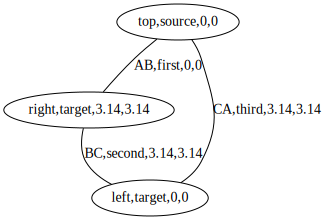
\includegraphics{save_custom_edges_and_vertices_graph_to_dot_test_custom_edges_and_vertices_k3_graph}

\caption{.svg file created from the create\_custom\_edges\_and\_vertices\_k3\_graph
function (algorithm \ref{alg:create_custom_edges_and_vertices_k3_graph})
and converted to .svg using the 'convert\_dot\_to\_svg' function (algorithm
\ref{alg:convert_dot_to_svg})\label{fig:save_custom_edges_and_vertices_graph_to_dot_test_custom_edges_and_vertices_k2_graph.svg}}
\end{figure}



\section{Other graph functions}


\subsection{Create an empty graph with a graph name property\label{sub:create_empty_directed_graph_with_graph_name}}

Algorithm \ref{alg:create_empty_directed_graph_with_graph_name} shows
the function to create an empty (directed) graph with a graph name.

\begin{algorithm}[H]
\lstinputlisting[breaklines=true,language={C++}]{create_empty_directed_graph_with_graph_name.impl}

\caption{Creating an empty directed graph with a graph name\index{create_empty_directed_graph_with_graph_name@create\_empty\_directed\_graph\_with\_graph\_name}\label{alg:create_empty_directed_graph_with_graph_name}}
\end{algorithm}


Algorithm \ref{alg:create_empty_directed_graph_with_graph_name_demo}
demonstrates the 'create\_empty\_directed\_graph\_with\_graph\_name'
function.

\begin{algorithm}[H]
\lstinputlisting[breaklines=true,language={C++}]{create_empty_directed_graph_with_graph_name_demo.impl}

\caption{Demonstration of 'create\_empty\_directed\_graph\_with\_graph\_name'\label{alg:create_empty_directed_graph_with_graph_name_demo}}
\end{algorithm}



\subsection{Set a graph its name property\label{sub:set_graph_name}}

If you know, please email me.

\begin{algorithm}[H]
\lstinputlisting[breaklines=true,language={C++}]{set_graph_name.impl}

\caption{Set a graph its name\index{set_graph_name@set\_graph\_name}\label{alg:set_graph_name}}
\end{algorithm}


Algorithm \ref{alg:set_graph_name_demo} demonstrates the 'set\_graph\_name'
function.

\begin{algorithm}[H]
\lstinputlisting[breaklines=true,language={C++}]{set_graph_name_demo.impl}

\caption{Demonstration of 'set\_graph\_name'\label{alg:set_graph_name_demo}}
\end{algorithm}



\subsection{Get a graph its name property\label{sub:get_graph_name}}

If you know, please email me.

\begin{algorithm}[H]
\lstinputlisting[breaklines=true,language={C++}]{get_graph_name.impl}

\caption{Get a graph its name\index{get_graph_name@get\_graph\_name}\label{alg:get_graph_name}}
\end{algorithm}


Algorithm \ref{alg:get_graph_name_demo} demonstrates the 'get\_graph\_name'
function.

\begin{algorithm}[H]
\lstinputlisting[breaklines=true,language={C++}]{get_graph_name_demo.impl}

\caption{Demonstration of 'get\_graph\_name'\label{alg:get_graph_name_demo}}
\end{algorithm}



\subsection{Create a K2 graph with a graph name property}

If you know, please email me.


\subsection{Storing a graph with a graph name property as a .dot}

If you know, please email me.


\section{Misc functions}

These are some function I needed for creating this tutorial. Although
they are not important for working with graphs, I used these heavily.
These functions may be compiler-dependent, platform-dependent and/or
there may be superior alternatives. I just add them for completeness.


\subsection{Getting a data type as a std::string\label{sub:get_type_name}}

This function will only work under GCC.

\begin{algorithm}[H]
\lstinputlisting[breaklines=true,language={C++}]{get_type_name.impl}

\caption{Getting a data type its name as a std::string\index{get_type_name@get\_type\_name}\label{alg:get_type_name}}
\end{algorithm}



\subsection{Convert a .dot to .svg\label{sub:convert_dot_to_svg}}

All illustrations in this tutorial are created by converting .dot
to a .svg ('Scalable Vector Graphic') file. This function assumes
the program 'dot' is installed, which is part of Graphviz.

\begin{algorithm}[H]
\lstinputlisting[breaklines=true,language={C++}]{convert_dot_to_svg.impl}

\caption{Convert a .dot file to a .svg\index{convert_dot_to_svg@convert\_dot\_to\_svg}\label{alg:convert_dot_to_svg}}
\end{algorithm}


'convert\_dot\_to\_svg' makes a system call to the prgram 'dot' to
convert the .dot file to an .svg file.


\subsection{Check if a file exists\label{sub:is_regular_file}}

Not the most smart way perhaps, but it does only use the STL.

\begin{algorithm}[H]
\lstinputlisting[breaklines=true,language={C++}]{is_regular_file.impl}

\caption{Check if a file exists\index{is_regular_file@is\_regular\_file}\label{alg:is_regular_file}}
\end{algorithm}



\section{Errors}

Some common errors.


\subsection{Formed reference to void\label{sub:formed_reference_to_void}}

This compile-time error occurs when you create a graph without a certain
property, then subsequently reading that property, as in algorithm
\ref{alg:formed_reference_to_void}: 

\begin{algorithm}[H]
\lstinputlisting[breaklines=true,language={C++}]{formed_reference_to_void.impl}

\caption{Creating the error 'formed reference to void'\index{formed_reference_to_void@formed\_reference\_to\_void}\label{alg:formed_reference_to_void}}
\end{algorithm}


In algorithm \ref{alg:formed_reference_to_void} a graph is created
with vertices of no properties. Then the names of these vertices,
which do not exists, are tried to be read. If you want to read the
names of the vertices, supply a graph that has this property.


\subsection{No matching function for call to 'clear\_out\_edges'\label{sub:no_matching_function_for_call_to_clear_out_edges}}

This compile-time error occurs when you want to clear the outward
edges from a vertex in an undirected graph. 

\begin{algorithm}[H]
\lstinputlisting[breaklines=true,language={C++}]{no_matching_function_for_call_to_clear_out_edges.impl}

\caption{Creating the error 'formed reference to void'\index{formed_reference_to_void@formed\_reference\_to\_void}\label{alg:no_matching_function_for_call_to_clear_out_edges}}
\end{algorithm}


In algorithm \ref{alg:no_matching_function_for_call_to_clear_out_edges}
an undirected graph is created, a vertex descriptor is obtained, then
its out edges are tried to be cleared. Either use a directed graph
(which has out edges), or use the 'boost::clear\_vertex' function
instead.


\subsection{No matching function for call to 'clear\_in\_edges'\label{sub:no_matching_function_for_call_to_clear_in_edges}}

See chapter \ref{sub:no_matching_function_for_call_to_clear_out_edges}.


\subsection{Undefined reference to boost::detail::graph::read\_graphviz\_new\label{sub:undefined_reference_to_read_graphviz_new}\index{read_graphviz_new@read\_graphviz\_new}}

You will have to link agains the Boost.Graph and Boost.Regex libraries.
In Qt Creator, this is achieved by adding these lines to your Qt Creator
project file:

\begin{lstlisting}
LIBS += -lboost_graph -lboost_regex 
\end{lstlisting}



\subsection{Property not found: node\_id\label{sub:property_not_found_node_id}\index{node_id@node\_id}\index{Propery not found}}

When loading a graph from file (as in chapter \ref{sub:load_undirected_graph_from_dot})
you will be using boost::read\_graphviz\index{boost::read_graphviz@boost::read\_graphviz}.
boost::read\_graphviz\index{boost::read_graphviz@boost::read\_graphviz}
needs a third argument, of type boost::dynamic\_properties\index{boost::dynamic_properties@boost::dynamic\_properties}.
When a graph does not have properties, do not use a default constructed
version, but initializate with 'boost::ignore\_other\_properties'\index{boost::ignore_other_properties@boost::ignore\_other\_properties}
as a constructor argument instead. Algorithm \ref{alg:property_not_found_node_id}
shows how to trigger this run-time error.

\begin{algorithm}[H]
\lstinputlisting[breaklines=true,language={C++}]{property_not_found_node_id.impl}

\caption{Storing a graph as a .dot file\index{save_graph_to_dot@save\_graph\_to\_dot}\label{alg:property_not_found_node_id}}
\end{algorithm}



\section{Appendix}


\subsection{List of all edge, graph and vertex properties\label{sub:all_properties}}

The following list is obtained from the file 'boost/graph/properties.hpp'.

\begin{tabular}{|c|c|c|}
\hline 
Edge & Graph & Vertex\tabularnewline
\hline 
\hline 
edge\_all & graph\_all & vertex\_all\tabularnewline
\hline 
edge\_bundle & graph\_bundle & vertex\_bundle\tabularnewline
\hline 
edge\_capacity & graph\_name & vertex\_centrality\tabularnewline
\hline 
edge\_centrality & graph\_visitor & vertex\_color\tabularnewline
\hline 
edge\_color &  & vertex\_current\_degree\tabularnewline
\hline 
edge\_discover\_time &  & vertex\_degree\tabularnewline
\hline 
edge\_finished &  & vertex\_discover\_time\tabularnewline
\hline 
edge\_flow &  & vertex\_distance\tabularnewline
\hline 
edge\_global &  & vertex\_distance2\tabularnewline
\hline 
edge\_index &  & vertex\_finish\_time\tabularnewline
\hline 
edge\_local &  & vertex\_global\tabularnewline
\hline 
edge\_local\_index &  & vertex\_in\_degree\tabularnewline
\hline 
edge\_name &  & vertex\_index\tabularnewline
\hline 
edge\_owner &  & vertex\_index1\tabularnewline
\hline 
edge\_residual\_capacity &  & vertex\_index2\tabularnewline
\hline 
edge\_reverse &  & vertex\_local\tabularnewline
\hline 
edge\_underlying &  & vertex\_local\_index\tabularnewline
\hline 
edge\_update &  & vertex\_lowpoint\tabularnewline
\hline 
edge\_weight &  & vertex\_name\tabularnewline
\hline 
edge\_weight2 &  & vertex\_out\_degree\tabularnewline
\hline 
 &  & vertex\_owner\tabularnewline
\hline 
 &  & vertex\_potential\tabularnewline
\hline 
 &  & vertex\_predecessor\tabularnewline
\hline 
 &  & vertex\_priority\tabularnewline
\hline 
 &  & vertex\_rank\tabularnewline
\hline 
 &  & vertex\_root\tabularnewline
\hline 
 &  & vertex\_underlying\tabularnewline
\hline 
 &  & vertex\_update\tabularnewline
\hline 
\end{tabular}

\bibliographystyle{plain}
\bibliography{boost_graph_tutorial}


\printindex{}
\end{document}
